\documentclass[twoside]{book}

% Packages required by doxygen
\usepackage{fixltx2e}
\usepackage{calc}
\usepackage{doxygen}
\usepackage[export]{adjustbox} % also loads graphicx
\usepackage{graphicx}
\usepackage[utf8]{inputenc}
\usepackage{makeidx}
\usepackage{multicol}
\usepackage{multirow}
\PassOptionsToPackage{warn}{textcomp}
\usepackage{textcomp}
\usepackage[nointegrals]{wasysym}
\usepackage[table]{xcolor}

% Font selection
\usepackage[T1]{fontenc}
\usepackage[scaled=.90]{helvet}
\usepackage{courier}
\usepackage{amssymb}
\usepackage{sectsty}
\renewcommand{\familydefault}{\sfdefault}
\allsectionsfont{%
  \fontseries{bc}\selectfont%
  \color{darkgray}%
}
\renewcommand{\DoxyLabelFont}{%
  \fontseries{bc}\selectfont%
  \color{darkgray}%
}
\newcommand{\+}{\discretionary{\mbox{\scriptsize$\hookleftarrow$}}{}{}}

% Page & text layout
\usepackage{geometry}
\geometry{%
  a4paper,%
  top=2.5cm,%
  bottom=2.5cm,%
  left=2.5cm,%
  right=2.5cm%
}
\tolerance=750
\hfuzz=15pt
\hbadness=750
\setlength{\emergencystretch}{15pt}
\setlength{\parindent}{0cm}
\setlength{\parskip}{0.2cm}
\makeatletter
\renewcommand{\paragraph}{%
  \@startsection{paragraph}{4}{0ex}{-1.0ex}{1.0ex}{%
    \normalfont\normalsize\bfseries\SS@parafont%
  }%
}
\renewcommand{\subparagraph}{%
  \@startsection{subparagraph}{5}{0ex}{-1.0ex}{1.0ex}{%
    \normalfont\normalsize\bfseries\SS@subparafont%
  }%
}
\makeatother

% Headers & footers
\usepackage{fancyhdr}
\pagestyle{fancyplain}
\fancyhead[LE]{\fancyplain{}{\bfseries\thepage}}
\fancyhead[CE]{\fancyplain{}{}}
\fancyhead[RE]{\fancyplain{}{\bfseries\leftmark}}
\fancyhead[LO]{\fancyplain{}{\bfseries\rightmark}}
\fancyhead[CO]{\fancyplain{}{}}
\fancyhead[RO]{\fancyplain{}{\bfseries\thepage}}
\fancyfoot[LE]{\fancyplain{}{}}
\fancyfoot[CE]{\fancyplain{}{}}
\fancyfoot[RE]{\fancyplain{}{\bfseries\scriptsize Generated by Doxygen }}
\fancyfoot[LO]{\fancyplain{}{\bfseries\scriptsize Generated by Doxygen }}
\fancyfoot[CO]{\fancyplain{}{}}
\fancyfoot[RO]{\fancyplain{}{}}
\renewcommand{\footrulewidth}{0.4pt}
\renewcommand{\chaptermark}[1]{%
  \markboth{#1}{}%
}
\renewcommand{\sectionmark}[1]{%
  \markright{\thesection\ #1}%
}

% Indices & bibliography
\usepackage{natbib}
\usepackage[titles]{tocloft}
\setcounter{tocdepth}{3}
\setcounter{secnumdepth}{5}
\makeindex

% Hyperlinks (required, but should be loaded last)
\usepackage{ifpdf}
\ifpdf
  \usepackage[pdftex,pagebackref=true]{hyperref}
\else
  \usepackage[ps2pdf,pagebackref=true]{hyperref}
\fi
\hypersetup{%
  colorlinks=true,%
  linkcolor=blue,%
  citecolor=blue,%
  unicode%
}

% Custom commands
\newcommand{\clearemptydoublepage}{%
  \newpage{\pagestyle{empty}\cleardoublepage}%
}


%===== C O N T E N T S =====

\begin{document}

% Titlepage & ToC
\hypersetup{pageanchor=false,
             bookmarks=true,
             bookmarksnumbered=true,
             pdfencoding=unicode
            }
\pagenumbering{roman}
\begin{titlepage}
\vspace*{7cm}
\begin{center}%
{\Large Glex \\[1ex]\large 2 }\\
\vspace*{1cm}
{\large Generated by Doxygen 1.8.10}\\
\end{center}
\end{titlepage}
\clearemptydoublepage
\tableofcontents
\clearemptydoublepage
\pagenumbering{arabic}
\hypersetup{pageanchor=true}

%--- Begin generated contents ---
\chapter{Namespace Index}
\section{Namespace List}
Here is a list of all namespaces with brief descriptions\+:\begin{DoxyCompactList}
\item\contentsline{section}{\hyperlink{namespace_python_b}{Python\+B} }{\pageref{namespace_python_b}}{}
\end{DoxyCompactList}

\chapter{Hierarchical Index}
\section{Class Hierarchy}
This inheritance list is sorted roughly, but not completely, alphabetically\+:\begin{DoxyCompactList}
\item \contentsline{section}{Bounding\+Box}{\pageref{class_bounding_box}}{}
\item \contentsline{section}{Camera}{\pageref{class_camera}}{}
\item \contentsline{section}{Game}{\pageref{class_game}}{}
\item \contentsline{section}{Game\+Asset}{\pageref{class_game_asset}}{}
\begin{DoxyCompactList}
\item \contentsline{section}{Cube\+Asset}{\pageref{class_cube_asset}}{}
\item \contentsline{section}{Floor\+Asset}{\pageref{class_floor_asset}}{}
\item \contentsline{section}{Pyramid\+Asset}{\pageref{class_pyramid_asset}}{}
\end{DoxyCompactList}
\item \contentsline{section}{Game\+Asset\+Manager}{\pageref{class_game_asset_manager}}{}
\item \contentsline{section}{Game\+World}{\pageref{class_game_world}}{}
\item \contentsline{section}{Python\+B}{\pageref{class_python_b}}{}
\item \contentsline{section}{S\+D\+L\+Window\+Deleter}{\pageref{struct_s_d_l_window_deleter}}{}
\end{DoxyCompactList}

\chapter{Class Index}
\section{Class List}
Here are the classes, structs, unions and interfaces with brief descriptions\+:\begin{DoxyCompactList}
\item\contentsline{section}{\hyperlink{classCubeAsset}{Cube\+Asset} }{\pageref{classCubeAsset}}{}
\item\contentsline{section}{\hyperlink{classFloorAsset}{Floor\+Asset} }{\pageref{classFloorAsset}}{}
\item\contentsline{section}{\hyperlink{classGameAsset}{Game\+Asset} }{\pageref{classGameAsset}}{}
\item\contentsline{section}{\hyperlink{classGameAssetManager}{Game\+Asset\+Manager} \\*\hyperlink{classGameAssetManager}{Game\+Asset\+Manager} is a container for Game\+Assets }{\pageref{classGameAssetManager}}{}
\item\contentsline{section}{\hyperlink{classGameWorld}{Game\+World} \\*\hyperlink{classGameWorld}{Game\+World} allows us to separate the management of the game world from the nuts and bolts of game loop initialisation }{\pageref{classGameWorld}}{}
\item\contentsline{section}{\hyperlink{classPyramidAsset}{Pyramid\+Asset} }{\pageref{classPyramidAsset}}{}
\item\contentsline{section}{\hyperlink{structSDLWindowDeleter}{S\+D\+L\+Window\+Deleter} }{\pageref{structSDLWindowDeleter}}{}
\end{DoxyCompactList}

\chapter{File Index}
\section{File List}
Here is a list of all files with brief descriptions\+:\begin{DoxyCompactList}
\item\contentsline{section}{\hyperlink{config_8h}{config.\+h} }{\pageref{config_8h}}{}
\item\contentsline{section}{src/\hyperlink{common_8h}{common.\+h} }{\pageref{common_8h}}{}
\item\contentsline{section}{src/\hyperlink{CubeAsset_8cc}{Cube\+Asset.\+cc} }{\pageref{CubeAsset_8cc}}{}
\item\contentsline{section}{src/\hyperlink{CubeAsset_8h}{Cube\+Asset.\+h} }{\pageref{CubeAsset_8h}}{}
\item\contentsline{section}{src/\hyperlink{FloorAsset_8cc}{Floor\+Asset.\+cc} }{\pageref{FloorAsset_8cc}}{}
\item\contentsline{section}{src/\hyperlink{FloorAsset_8h}{Floor\+Asset.\+h} }{\pageref{FloorAsset_8h}}{}
\item\contentsline{section}{src/\hyperlink{GameAsset_8h}{Game\+Asset.\+h} }{\pageref{GameAsset_8h}}{}
\item\contentsline{section}{src/\hyperlink{GameAssetManager_8cc}{Game\+Asset\+Manager.\+cc} }{\pageref{GameAssetManager_8cc}}{}
\item\contentsline{section}{src/\hyperlink{GameAssetManager_8h}{Game\+Asset\+Manager.\+h} }{\pageref{GameAssetManager_8h}}{}
\item\contentsline{section}{src/\hyperlink{GameWorld_8cc}{Game\+World.\+cc} }{\pageref{GameWorld_8cc}}{}
\item\contentsline{section}{src/\hyperlink{GameWorld_8h}{Game\+World.\+h} }{\pageref{GameWorld_8h}}{}
\item\contentsline{section}{src/\hyperlink{main_8cc}{main.\+cc} }{\pageref{main_8cc}}{}
\item\contentsline{section}{src/\hyperlink{PyramidAsset_8cc}{Pyramid\+Asset.\+cc} }{\pageref{PyramidAsset_8cc}}{}
\item\contentsline{section}{src/\hyperlink{PyramidAsset_8h}{Pyramid\+Asset.\+h} }{\pageref{PyramidAsset_8h}}{}
\end{DoxyCompactList}

\chapter{Namespace Documentation}
\hypertarget{namespace_python_b}{}\section{Python\+B Namespace Reference}
\label{namespace_python_b}\index{Python\+B@{Python\+B}}

\chapter{Class Documentation}
\hypertarget{class_bounding_box}{}\section{Bounding\+Box Class Reference}
\label{class_bounding_box}\index{Bounding\+Box@{Bounding\+Box}}


{\ttfamily \#include $<$Bounding\+Box.\+h$>$}

\subsection*{Public Member Functions}
\begin{DoxyCompactItemize}
\item 
\hyperlink{class_bounding_box_afb9207b7a7e84a20c48e02914ce73253}{Bounding\+Box} (glm\+::vec3 Spawn, glm\+::vec3 xyz\+Pos, glm\+::vec3 xyz\+Translation, bool xyz\+Tbool)
\item 
glm\+::mat4 \hyperlink{class_bounding_box_a5fd1769f7157e7df40a6ab6a242fcfcc}{Get\+Model} ()
\item 
void \hyperlink{class_bounding_box_a698cfa6bf6412b7b9f7ebe78ababa339}{Translate} ()
\end{DoxyCompactItemize}


\subsection{Constructor \& Destructor Documentation}
\hypertarget{class_bounding_box_afb9207b7a7e84a20c48e02914ce73253}{}\index{Bounding\+Box@{Bounding\+Box}!Bounding\+Box@{Bounding\+Box}}
\index{Bounding\+Box@{Bounding\+Box}!Bounding\+Box@{Bounding\+Box}}
\subsubsection[{Bounding\+Box(glm\+::vec3 Spawn, glm\+::vec3 xyz\+Pos, glm\+::vec3 xyz\+Translation, bool xyz\+Tbool)}]{\setlength{\rightskip}{0pt plus 5cm}Bounding\+Box\+::\+Bounding\+Box (
\begin{DoxyParamCaption}
\item[{glm\+::vec3}]{Spawn, }
\item[{glm\+::vec3}]{xyz\+Pos, }
\item[{glm\+::vec3}]{xyz\+Translation, }
\item[{bool}]{xyz\+Tbool}
\end{DoxyParamCaption}
)}\label{class_bounding_box_afb9207b7a7e84a20c48e02914ce73253}
\hyperlink{class_bounding_box}{Bounding\+Box} Using glm vectors to store the xyz co-\/ordinates. initialises the points using \char`\"{}this\char`\"{} keyword. Tpoint is used for the translation point. 

\subsection{Member Function Documentation}
\hypertarget{class_bounding_box_a5fd1769f7157e7df40a6ab6a242fcfcc}{}\index{Bounding\+Box@{Bounding\+Box}!Get\+Model@{Get\+Model}}
\index{Get\+Model@{Get\+Model}!Bounding\+Box@{Bounding\+Box}}
\subsubsection[{Get\+Model()}]{\setlength{\rightskip}{0pt plus 5cm}glm\+::mat4 Bounding\+Box\+::\+Get\+Model (
\begin{DoxyParamCaption}
{}
\end{DoxyParamCaption}
)}\label{class_bounding_box_a5fd1769f7157e7df40a6ab6a242fcfcc}
Get Model (C\+H\+A\+N\+G\+E) This gets the Model Matrics. 

Here is the call graph for this function\+:
\nopagebreak
\begin{figure}[H]
\begin{center}
\leavevmode
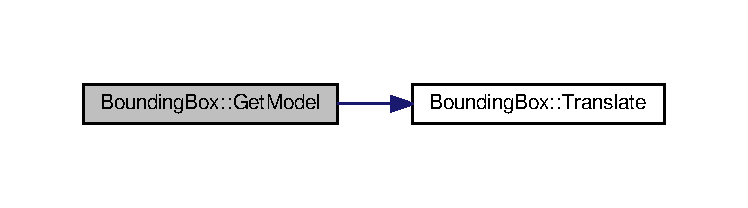
\includegraphics[width=350pt]{class_bounding_box_a5fd1769f7157e7df40a6ab6a242fcfcc_cgraph}
\end{center}
\end{figure}


\hypertarget{class_bounding_box_a698cfa6bf6412b7b9f7ebe78ababa339}{}\index{Bounding\+Box@{Bounding\+Box}!Translate@{Translate}}
\index{Translate@{Translate}!Bounding\+Box@{Bounding\+Box}}
\subsubsection[{Translate()}]{\setlength{\rightskip}{0pt plus 5cm}void Bounding\+Box\+::\+Translate (
\begin{DoxyParamCaption}
{}
\end{DoxyParamCaption}
)}\label{class_bounding_box_a698cfa6bf6412b7b9f7ebe78ababa339}
Translate Method Used for translation animation. Moves the asset based on the x, y and/or z axis. 

Here is the caller graph for this function\+:
\nopagebreak
\begin{figure}[H]
\begin{center}
\leavevmode
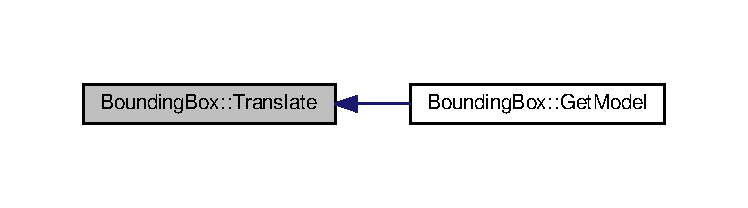
\includegraphics[width=350pt]{class_bounding_box_a698cfa6bf6412b7b9f7ebe78ababa339_icgraph}
\end{center}
\end{figure}




The documentation for this class was generated from the following files\+:\begin{DoxyCompactItemize}
\item 
src/\hyperlink{_bounding_box_8h}{Bounding\+Box.\+h}\item 
src/\hyperlink{_bounding_box_8cc}{Bounding\+Box.\+cc}\end{DoxyCompactItemize}

\hypertarget{class_camera}{}\section{Camera Class Reference}
\label{class_camera}\index{Camera@{Camera}}


{\ttfamily \#include $<$Camera.\+h$>$}

\subsection*{Public Member Functions}
\begin{DoxyCompactItemize}
\item 
\hyperlink{class_camera_a01f94c3543f56ede7af49dc778f19331}{Camera} ()
\item 
glm\+::mat4 \hyperlink{class_camera_ac0f7e4d6a41e3b425eed9cfa392a9508}{Update\+Camera\+Position} (\hyperlink{common_8h_a080a822f0093973313bd644e517a5090}{Input} input\+\_\+\+Direction, int mouse\+X, int mouse\+Y)
\end{DoxyCompactItemize}


\subsection{Constructor \& Destructor Documentation}
\hypertarget{class_camera_a01f94c3543f56ede7af49dc778f19331}{}\index{Camera@{Camera}!Camera@{Camera}}
\index{Camera@{Camera}!Camera@{Camera}}
\subsubsection[{Camera()}]{\setlength{\rightskip}{0pt plus 5cm}Camera\+::\+Camera (
\begin{DoxyParamCaption}
{}
\end{DoxyParamCaption}
)}\label{class_camera_a01f94c3543f56ede7af49dc778f19331}
based on the tutorial found here\+: \href{http://www.opengl-tutorial.org/beginners-tutorials/tutorial-6-keyboard-and-mouse/}{\tt http\+://www.\+opengl-\/tutorial.\+org/beginners-\/tutorials/tutorial-\/6-\/keyboard-\/and-\/mouse/} results in a camera that follows an axis 

\subsection{Member Function Documentation}
\hypertarget{class_camera_ac0f7e4d6a41e3b425eed9cfa392a9508}{}\index{Camera@{Camera}!Update\+Camera\+Position@{Update\+Camera\+Position}}
\index{Update\+Camera\+Position@{Update\+Camera\+Position}!Camera@{Camera}}
\subsubsection[{Update\+Camera\+Position(\+Input input\+\_\+\+Direction, int mouse\+X, int mouse\+Y)}]{\setlength{\rightskip}{0pt plus 5cm}glm\+::mat4 Camera\+::\+Update\+Camera\+Position (
\begin{DoxyParamCaption}
\item[{{\bf Input}}]{input\+\_\+\+Direction, }
\item[{int}]{mouse\+X, }
\item[{int}]{mouse\+Y}
\end{DoxyParamCaption}
)}\label{class_camera_ac0f7e4d6a41e3b425eed9cfa392a9508}
Update \hyperlink{class_camera}{Camera} Position Key control is I\+N\+D\+E\+P\+E\+N\+D\+E\+N\+T of camera direction. Mouse position is updated using the inverse of the x and y positions. Uses the Keyboard inputs from the main. Calculates the direction, the travel right and the travel up. These are inverted to get left and down travel.

Here is the caller graph for this function\+:
\nopagebreak
\begin{figure}[H]
\begin{center}
\leavevmode
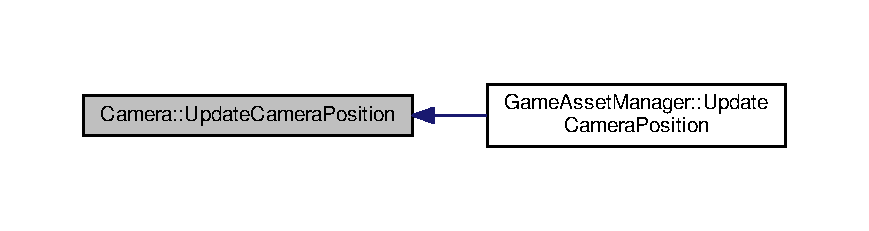
\includegraphics[width=350pt]{class_camera_ac0f7e4d6a41e3b425eed9cfa392a9508_icgraph}
\end{center}
\end{figure}




The documentation for this class was generated from the following files\+:\begin{DoxyCompactItemize}
\item 
src/\hyperlink{_camera_8h}{Camera.\+h}\item 
src/\hyperlink{_camera_8cc}{Camera.\+cc}\end{DoxyCompactItemize}

\hypertarget{class_cube_asset}{}\section{Cube\+Asset Class Reference}
\label{class_cube_asset}\index{Cube\+Asset@{Cube\+Asset}}


{\ttfamily \#include $<$Cube\+Asset.\+h$>$}



Inheritance diagram for Cube\+Asset\+:
\nopagebreak
\begin{figure}[H]
\begin{center}
\leavevmode
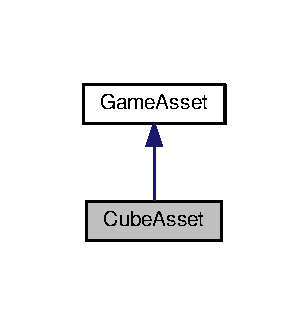
\includegraphics[width=148pt]{class_cube_asset__inherit__graph}
\end{center}
\end{figure}


Collaboration diagram for Cube\+Asset\+:
\nopagebreak
\begin{figure}[H]
\begin{center}
\leavevmode
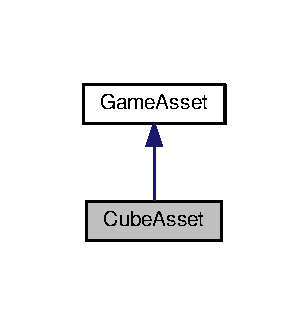
\includegraphics[width=148pt]{class_cube_asset__coll__graph}
\end{center}
\end{figure}
\subsection*{Public Member Functions}
\begin{DoxyCompactItemize}
\item 
\hyperlink{class_cube_asset_a0e4fb8ef862794c7c86e8dbfc5f39b59}{Cube\+Asset} (glm\+::vec3 Spawn, glm\+::vec3 xyz\+Pos, glm\+::vec3 xyz\+Translation, bool xyz\+Tbool)
\item 
\hyperlink{class_cube_asset_ab3ab9a5da82cbf8537a28652410093b1}{$\sim$\+Cube\+Asset} ()
\item 
virtual void \hyperlink{class_cube_asset_a1af568486056e254ffcf98fd99947bfe}{Draw} (G\+Luint)
\end{DoxyCompactItemize}


\subsection{Constructor \& Destructor Documentation}
\hypertarget{class_cube_asset_a0e4fb8ef862794c7c86e8dbfc5f39b59}{}\index{Cube\+Asset@{Cube\+Asset}!Cube\+Asset@{Cube\+Asset}}
\index{Cube\+Asset@{Cube\+Asset}!Cube\+Asset@{Cube\+Asset}}
\subsubsection[{Cube\+Asset(glm\+::vec3 Spawn, glm\+::vec3 xyz\+Pos, glm\+::vec3 xyz\+Translation, bool xyz\+Tbool)}]{\setlength{\rightskip}{0pt plus 5cm}Cube\+Asset\+::\+Cube\+Asset (
\begin{DoxyParamCaption}
\item[{glm\+::vec3}]{Spawn, }
\item[{glm\+::vec3}]{xyz\+Pos, }
\item[{glm\+::vec3}]{xyz\+Translation, }
\item[{bool}]{xyz\+Tbool}
\end{DoxyParamCaption}
)}\label{class_cube_asset_a0e4fb8ef862794c7c86e8dbfc5f39b59}
Cube Creation models coordinates, origin dependant on xyz variables. vertex buffer models coordinates, for the triangles. colour buffer models the colour of the object triangles. element buffer creates the cube using 12 triangles.

Buffer Implementation Transfer buffers to the G\+P\+U\hypertarget{class_cube_asset_ab3ab9a5da82cbf8537a28652410093b1}{}\index{Cube\+Asset@{Cube\+Asset}!````~Cube\+Asset@{$\sim$\+Cube\+Asset}}
\index{````~Cube\+Asset@{$\sim$\+Cube\+Asset}!Cube\+Asset@{Cube\+Asset}}
\subsubsection[{$\sim$\+Cube\+Asset()}]{\setlength{\rightskip}{0pt plus 5cm}Cube\+Asset\+::$\sim$\+Cube\+Asset (
\begin{DoxyParamCaption}
{}
\end{DoxyParamCaption}
)}\label{class_cube_asset_ab3ab9a5da82cbf8537a28652410093b1}


\subsection{Member Function Documentation}
\hypertarget{class_cube_asset_a1af568486056e254ffcf98fd99947bfe}{}\index{Cube\+Asset@{Cube\+Asset}!Draw@{Draw}}
\index{Draw@{Draw}!Cube\+Asset@{Cube\+Asset}}
\subsubsection[{Draw(\+G\+Luint)}]{\setlength{\rightskip}{0pt plus 5cm}void Cube\+Asset\+::\+Draw (
\begin{DoxyParamCaption}
\item[{G\+Luint}]{program\+\_\+token}
\end{DoxyParamCaption}
)\hspace{0.3cm}{\ttfamily [virtual]}}\label{class_cube_asset_a1af568486056e254ffcf98fd99947bfe}
Buffer Arrays use the previously transferred buffer as the vertex array. This way we transfer the buffer once -- at construction -- not on every frame.

Implements \hyperlink{class_game_asset_a961aa51ca0a9961fc584c0b5d5431300}{Game\+Asset}.



The documentation for this class was generated from the following files\+:\begin{DoxyCompactItemize}
\item 
src/\hyperlink{_cube_asset_8h}{Cube\+Asset.\+h}\item 
src/\hyperlink{_cube_asset_8cc}{Cube\+Asset.\+cc}\end{DoxyCompactItemize}

\hypertarget{class_floor_asset}{}\section{Floor\+Asset Class Reference}
\label{class_floor_asset}\index{Floor\+Asset@{Floor\+Asset}}


{\ttfamily \#include $<$Floor\+Asset.\+h$>$}



Inheritance diagram for Floor\+Asset\+:
\nopagebreak
\begin{figure}[H]
\begin{center}
\leavevmode
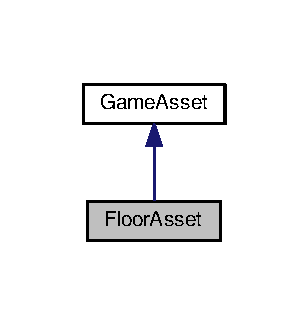
\includegraphics[width=148pt]{class_floor_asset__inherit__graph}
\end{center}
\end{figure}


Collaboration diagram for Floor\+Asset\+:
\nopagebreak
\begin{figure}[H]
\begin{center}
\leavevmode
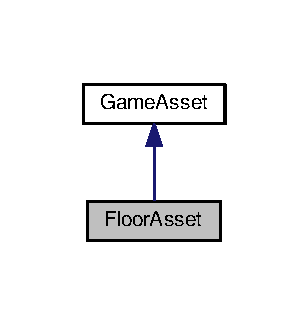
\includegraphics[width=148pt]{class_floor_asset__coll__graph}
\end{center}
\end{figure}
\subsection*{Public Member Functions}
\begin{DoxyCompactItemize}
\item 
\hyperlink{class_floor_asset_a4b8e3fb6415ed1126c9243267c7195a8}{Floor\+Asset} (glm\+::vec3 Spawn, glm\+::vec3 xyz\+Pos, glm\+::vec3 xyz\+Translation, bool xyz\+Tbool)
\item 
\hyperlink{class_floor_asset_a7d782882bb08ee2a2285821275383856}{$\sim$\+Floor\+Asset} ()
\item 
virtual void \hyperlink{class_floor_asset_a14650eb2c2cd75e990c351bad8636279}{Draw} (G\+Luint)
\end{DoxyCompactItemize}


\subsection{Constructor \& Destructor Documentation}
\hypertarget{class_floor_asset_a4b8e3fb6415ed1126c9243267c7195a8}{}\index{Floor\+Asset@{Floor\+Asset}!Floor\+Asset@{Floor\+Asset}}
\index{Floor\+Asset@{Floor\+Asset}!Floor\+Asset@{Floor\+Asset}}
\subsubsection[{Floor\+Asset(glm\+::vec3 Spawn, glm\+::vec3 xyz\+Pos, glm\+::vec3 xyz\+Translation, bool xyz\+Tbool)}]{\setlength{\rightskip}{0pt plus 5cm}Floor\+Asset\+::\+Floor\+Asset (
\begin{DoxyParamCaption}
\item[{glm\+::vec3}]{Spawn, }
\item[{glm\+::vec3}]{xyz\+Pos, }
\item[{glm\+::vec3}]{xyz\+Translation, }
\item[{bool}]{xyz\+Tbool}
\end{DoxyParamCaption}
)}\label{class_floor_asset_a4b8e3fb6415ed1126c9243267c7195a8}
Cube Creation This uses the same definitions as \hyperlink{class_cube_asset}{Cube\+Asset} with different coordinates. models coordinates, origin dependant on xyz variables. vertex buffer models coordinates, for the triangles. colour buffer models the colour of the object triangles. element buffer creates the cube using 12 triangles.

Buffer Implementation Transfer buffers to the G\+P\+U\hypertarget{class_floor_asset_a7d782882bb08ee2a2285821275383856}{}\index{Floor\+Asset@{Floor\+Asset}!````~Floor\+Asset@{$\sim$\+Floor\+Asset}}
\index{````~Floor\+Asset@{$\sim$\+Floor\+Asset}!Floor\+Asset@{Floor\+Asset}}
\subsubsection[{$\sim$\+Floor\+Asset()}]{\setlength{\rightskip}{0pt plus 5cm}Floor\+Asset\+::$\sim$\+Floor\+Asset (
\begin{DoxyParamCaption}
{}
\end{DoxyParamCaption}
)}\label{class_floor_asset_a7d782882bb08ee2a2285821275383856}


\subsection{Member Function Documentation}
\hypertarget{class_floor_asset_a14650eb2c2cd75e990c351bad8636279}{}\index{Floor\+Asset@{Floor\+Asset}!Draw@{Draw}}
\index{Draw@{Draw}!Floor\+Asset@{Floor\+Asset}}
\subsubsection[{Draw(\+G\+Luint)}]{\setlength{\rightskip}{0pt plus 5cm}void Floor\+Asset\+::\+Draw (
\begin{DoxyParamCaption}
\item[{G\+Luint}]{program\+\_\+token}
\end{DoxyParamCaption}
)\hspace{0.3cm}{\ttfamily [virtual]}}\label{class_floor_asset_a14650eb2c2cd75e990c351bad8636279}
Buffer Arrays use the previously transferred buffer as the vertex array. This way we transfer the buffer once -- at construction -- not on every frame.

Implements \hyperlink{class_game_asset_a961aa51ca0a9961fc584c0b5d5431300}{Game\+Asset}.



The documentation for this class was generated from the following files\+:\begin{DoxyCompactItemize}
\item 
src/\hyperlink{_floor_asset_8h}{Floor\+Asset.\+h}\item 
src/\hyperlink{_floor_asset_8cc}{Floor\+Asset.\+cc}\end{DoxyCompactItemize}

\hypertarget{class_game}{}\section{Game Class Reference}
\label{class_game}\index{Game@{Game}}


{\ttfamily \#include $<$Game.\+h$>$}

\subsection*{Public Member Functions}
\begin{DoxyCompactItemize}
\item 
std\+::shared\+\_\+ptr$<$ S\+D\+L\+\_\+\+Window $>$ \hyperlink{class_game_aa12ca9a4e954b358cc4cdaf059c4485e}{Init\+World} ()
\item 
void \hyperlink{class_game_aafad890eae2f5627f55fffc0b6e12b58}{Draw} (const std\+::shared\+\_\+ptr$<$ S\+D\+L\+\_\+\+Window $>$ \&window, const std\+::shared\+\_\+ptr$<$ \hyperlink{class_game_world}{Game\+World} $>$ \&game\+\_\+world)
\item 
void \hyperlink{class_game_adb05b20574551a26f8cf1dc664782790}{Start} ()
\end{DoxyCompactItemize}


\subsection{Member Function Documentation}
\hypertarget{class_game_aafad890eae2f5627f55fffc0b6e12b58}{}\index{Game@{Game}!Draw@{Draw}}
\index{Draw@{Draw}!Game@{Game}}
\subsubsection[{Draw(const std\+::shared\+\_\+ptr$<$ S\+D\+L\+\_\+\+Window $>$ \&window, const std\+::shared\+\_\+ptr$<$ Game\+World $>$ \&game\+\_\+world)}]{\setlength{\rightskip}{0pt plus 5cm}void Game\+::\+Draw (
\begin{DoxyParamCaption}
\item[{const std\+::shared\+\_\+ptr$<$ S\+D\+L\+\_\+\+Window $>$ \&}]{window, }
\item[{const std\+::shared\+\_\+ptr$<$ {\bf Game\+World} $>$ \&}]{game\+\_\+world}
\end{DoxyParamCaption}
)}\label{class_game_aafad890eae2f5627f55fffc0b6e12b58}


Here is the caller graph for this function\+:\nopagebreak
\begin{figure}[H]
\begin{center}
\leavevmode
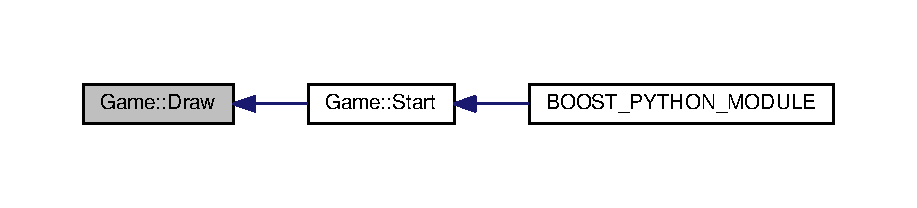
\includegraphics[width=350pt]{class_game_aafad890eae2f5627f55fffc0b6e12b58_icgraph}
\end{center}
\end{figure}


\hypertarget{class_game_aa12ca9a4e954b358cc4cdaf059c4485e}{}\index{Game@{Game}!Init\+World@{Init\+World}}
\index{Init\+World@{Init\+World}!Game@{Game}}
\subsubsection[{Init\+World()}]{\setlength{\rightskip}{0pt plus 5cm}std\+::shared\+\_\+ptr$<$ S\+D\+L\+\_\+\+Window $>$ Game\+::\+Init\+World (
\begin{DoxyParamCaption}
{}
\end{DoxyParamCaption}
)}\label{class_game_aa12ca9a4e954b358cc4cdaf059c4485e}
Initialise G\+L\+E\+W -\/ an easy way to ensure Open\+Gl 3.\+0+ The {\itshape must} be done after we have set the video mode -\/ otherwise we have no Open\+G\+L context to test.

Here is the caller graph for this function\+:\nopagebreak
\begin{figure}[H]
\begin{center}
\leavevmode
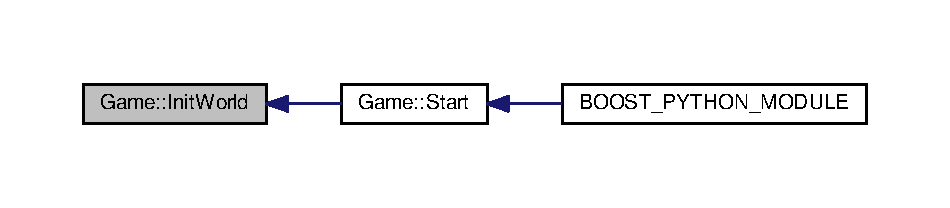
\includegraphics[width=350pt]{class_game_aa12ca9a4e954b358cc4cdaf059c4485e_icgraph}
\end{center}
\end{figure}


\hypertarget{class_game_adb05b20574551a26f8cf1dc664782790}{}\index{Game@{Game}!Start@{Start}}
\index{Start@{Start}!Game@{Game}}
\subsubsection[{Start()}]{\setlength{\rightskip}{0pt plus 5cm}void Game\+::\+Start (
\begin{DoxyParamCaption}
{}
\end{DoxyParamCaption}
)}\label{class_game_adb05b20574551a26f8cf1dc664782790}
Inputs S\+D\+L Inputs for Mouse working on the x and y. S\+D\+L keyboard Inputs which are later sent to the \hyperlink{class_camera}{Camera} Class. Keyboard uses \char`\"{}\+W,\+A,\+S,\+D\char`\"{} formation over arrows keys. Whilst J,K are used for Ascend and Descend

Here is the call graph for this function\+:\nopagebreak
\begin{figure}[H]
\begin{center}
\leavevmode
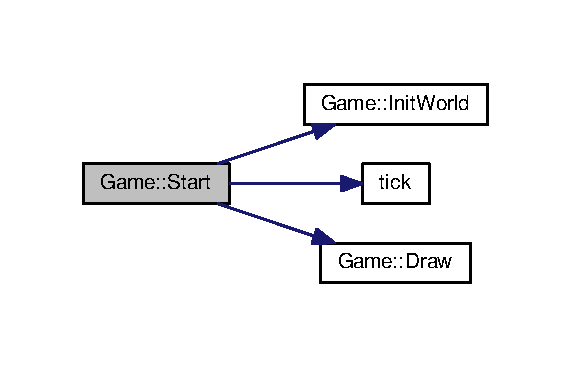
\includegraphics[width=274pt]{class_game_adb05b20574551a26f8cf1dc664782790_cgraph}
\end{center}
\end{figure}




Here is the caller graph for this function\+:\nopagebreak
\begin{figure}[H]
\begin{center}
\leavevmode
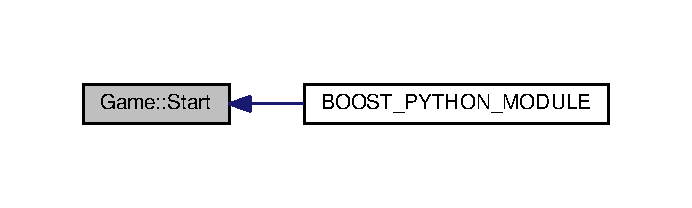
\includegraphics[width=332pt]{class_game_adb05b20574551a26f8cf1dc664782790_icgraph}
\end{center}
\end{figure}




The documentation for this class was generated from the following files\+:\begin{DoxyCompactItemize}
\item 
src/\hyperlink{_game_8h}{Game.\+h}\item 
src/\hyperlink{_game_8cc}{Game.\+cc}\end{DoxyCompactItemize}

\hypertarget{class_game_asset}{}\section{Game\+Asset Class Reference}
\label{class_game_asset}\index{Game\+Asset@{Game\+Asset}}


{\ttfamily \#include $<$Game\+Asset.\+h$>$}



Inheritance diagram for Game\+Asset\+:\nopagebreak
\begin{figure}[H]
\begin{center}
\leavevmode
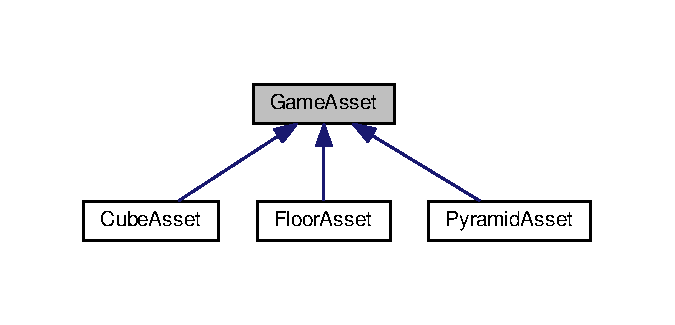
\includegraphics[width=324pt]{class_game_asset__inherit__graph}
\end{center}
\end{figure}
\subsection*{Public Member Functions}
\begin{DoxyCompactItemize}
\item 
\hyperlink{class_game_asset_a528ae8efd37541dc4c5a2ad643807e51}{Game\+Asset} (glm\+::vec3 Spawn, glm\+::vec3 xyz\+Pos, glm\+::vec3 xyz\+Translation, bool xyz\+Tbool)
\item 
glm\+::mat4 \hyperlink{class_game_asset_a50a4795382fb55c7513314f82821e444}{Get\+Model} ()
\item 
virtual void \hyperlink{class_game_asset_a961aa51ca0a9961fc584c0b5d5431300}{Draw} (G\+Luint)=0
\end{DoxyCompactItemize}


\subsection{Constructor \& Destructor Documentation}
\hypertarget{class_game_asset_a528ae8efd37541dc4c5a2ad643807e51}{}\index{Game\+Asset@{Game\+Asset}!Game\+Asset@{Game\+Asset}}
\index{Game\+Asset@{Game\+Asset}!Game\+Asset@{Game\+Asset}}
\subsubsection[{Game\+Asset(glm\+::vec3 Spawn, glm\+::vec3 xyz\+Pos, glm\+::vec3 xyz\+Translation, bool xyz\+Tbool)}]{\setlength{\rightskip}{0pt plus 5cm}Game\+Asset\+::\+Game\+Asset (
\begin{DoxyParamCaption}
\item[{glm\+::vec3}]{Spawn, }
\item[{glm\+::vec3}]{xyz\+Pos, }
\item[{glm\+::vec3}]{xyz\+Translation, }
\item[{bool}]{xyz\+Tbool}
\end{DoxyParamCaption}
)}\label{class_game_asset_a528ae8efd37541dc4c5a2ad643807e51}
{\itshape C\+H\+A\+N\+G\+E M\+E} Send Data To Bounding Box This Method Sends all the Data from spawning the Asset and sends it to the Bounding Box Class to create the Bounding Box and Manipulate the Asset 

\subsection{Member Function Documentation}
\hypertarget{class_game_asset_a961aa51ca0a9961fc584c0b5d5431300}{}\index{Game\+Asset@{Game\+Asset}!Draw@{Draw}}
\index{Draw@{Draw}!Game\+Asset@{Game\+Asset}}
\subsubsection[{Draw(\+G\+Luint)=0}]{\setlength{\rightskip}{0pt plus 5cm}virtual void Game\+Asset\+::\+Draw (
\begin{DoxyParamCaption}
\item[{G\+Luint}]{}
\end{DoxyParamCaption}
)\hspace{0.3cm}{\ttfamily [pure virtual]}}\label{class_game_asset_a961aa51ca0a9961fc584c0b5d5431300}


Implemented in \hyperlink{class_cube_asset_a1af568486056e254ffcf98fd99947bfe}{Cube\+Asset}, \hyperlink{class_floor_asset_a14650eb2c2cd75e990c351bad8636279}{Floor\+Asset}, and \hyperlink{class_pyramid_asset_aaea45da4956d79ec9ab96e9d0ccef3fe}{Pyramid\+Asset}.

\hypertarget{class_game_asset_a50a4795382fb55c7513314f82821e444}{}\index{Game\+Asset@{Game\+Asset}!Get\+Model@{Get\+Model}}
\index{Get\+Model@{Get\+Model}!Game\+Asset@{Game\+Asset}}
\subsubsection[{Get\+Model()}]{\setlength{\rightskip}{0pt plus 5cm}glm\+::mat4 Game\+Asset\+::\+Get\+Model (
\begin{DoxyParamCaption}
{}
\end{DoxyParamCaption}
)}\label{class_game_asset_a50a4795382fb55c7513314f82821e444}
{\itshape C\+H\+A\+N\+G\+E M\+E} Get Model This class Gets the Model from the Bounding Box class, This method is normally called by the Draw method in \hyperlink{class_game_asset_manager}{Game\+Asset\+Manager} 

The documentation for this class was generated from the following files\+:\begin{DoxyCompactItemize}
\item 
src/\hyperlink{_game_asset_8h}{Game\+Asset.\+h}\item 
src/\hyperlink{_game_asset_8cc}{Game\+Asset.\+cc}\end{DoxyCompactItemize}

\hypertarget{class_game_asset_manager}{}\section{Game\+Asset\+Manager Class Reference}
\label{class_game_asset_manager}\index{Game\+Asset\+Manager@{Game\+Asset\+Manager}}


{\ttfamily \#include $<$Game\+Asset\+Manager.\+h$>$}

\subsection*{Public Member Functions}
\begin{DoxyCompactItemize}
\item 
\hyperlink{class_game_asset_manager_a84d0445928649e0d1e0f8e31ee137b17}{Game\+Asset\+Manager} ()
\begin{DoxyCompactList}\small\item\em Creates a \hyperlink{class_game_asset_manager}{Game\+Asset\+Manager} to load the correct shaders. \end{DoxyCompactList}\item 
virtual \hyperlink{class_game_asset_manager_a1270bd61ecbcca563f079803e40c9b77}{$\sim$\+Game\+Asset\+Manager} ()
\item 
\hyperlink{class_game_asset_manager_a2c9adcb72faa154c87eadc9bafe5269d}{Game\+Asset\+Manager} (\hyperlink{class_game_asset_manager}{Game\+Asset\+Manager} const \&)
\item 
\hyperlink{class_game_asset_manager_a44f6e2fd6b8ff1dd64e5697f1be7386d}{Game\+Asset\+Manager} (\hyperlink{class_game_asset_manager}{Game\+Asset\+Manager} const \&\&)
\item 
void \hyperlink{class_game_asset_manager_a7c9e4fce50b47b78652e7ff0b4dbb629}{operator=} (\hyperlink{class_game_asset_manager}{Game\+Asset\+Manager})
\item 
void \hyperlink{class_game_asset_manager_ad3de8ff00d55ba04728b1de8213b2349}{Add\+Asset} (std\+::shared\+\_\+ptr$<$ \hyperlink{class_game_asset}{Game\+Asset} $>$)
\begin{DoxyCompactList}\small\item\em Adds a \hyperlink{class_game_asset}{Game\+Asset} to the scene graph. \end{DoxyCompactList}\item 
void \hyperlink{class_game_asset_manager_a32837132bd70a9a9ed537323c2d3d886}{Draw} ()
\begin{DoxyCompactList}\small\item\em Draws each \hyperlink{class_game_asset}{Game\+Asset} in the scene graph. \end{DoxyCompactList}\item 
void \hyperlink{class_game_asset_manager_afbcf9d370cfefc67a696395f2cdf1a9b}{Update\+Camera\+Position} (\hyperlink{common_8h_a080a822f0093973313bd644e517a5090}{Input} input\+\_\+\+Direction, int mouse\+X, int mouse\+Y)
\end{DoxyCompactItemize}


\subsection{Detailed Description}
\hyperlink{class_game_asset_manager}{Game\+Asset\+Manager} is a container for Game\+Assets. It also provides utility functions to to create a simple Open\+G\+L program that can be used to draw a simple \hyperlink{class_game_asset}{Game\+Asset}. 

\subsection{Constructor \& Destructor Documentation}
\hypertarget{class_game_asset_manager_a84d0445928649e0d1e0f8e31ee137b17}{}\index{Game\+Asset\+Manager@{Game\+Asset\+Manager}!Game\+Asset\+Manager@{Game\+Asset\+Manager}}
\index{Game\+Asset\+Manager@{Game\+Asset\+Manager}!Game\+Asset\+Manager@{Game\+Asset\+Manager}}
\subsubsection[{Game\+Asset\+Manager()}]{\setlength{\rightskip}{0pt plus 5cm}Game\+Asset\+Manager\+::\+Game\+Asset\+Manager (
\begin{DoxyParamCaption}
{}
\end{DoxyParamCaption}
)\hspace{0.3cm}{\ttfamily [explicit]}}\label{class_game_asset_manager_a84d0445928649e0d1e0f8e31ee137b17}


Creates a \hyperlink{class_game_asset_manager}{Game\+Asset\+Manager} to load the correct shaders. 

\hypertarget{class_game_asset_manager_a1270bd61ecbcca563f079803e40c9b77}{}\index{Game\+Asset\+Manager@{Game\+Asset\+Manager}!````~Game\+Asset\+Manager@{$\sim$\+Game\+Asset\+Manager}}
\index{````~Game\+Asset\+Manager@{$\sim$\+Game\+Asset\+Manager}!Game\+Asset\+Manager@{Game\+Asset\+Manager}}
\subsubsection[{$\sim$\+Game\+Asset\+Manager()}]{\setlength{\rightskip}{0pt plus 5cm}Game\+Asset\+Manager\+::$\sim$\+Game\+Asset\+Manager (
\begin{DoxyParamCaption}
{}
\end{DoxyParamCaption}
)\hspace{0.3cm}{\ttfamily [virtual]}}\label{class_game_asset_manager_a1270bd61ecbcca563f079803e40c9b77}
Deletes a \hyperlink{class_game_asset_manager}{Game\+Asset\+Manager}, in particular it will clean up any modifications to the Open\+G\+L state. \hypertarget{class_game_asset_manager_a2c9adcb72faa154c87eadc9bafe5269d}{}\index{Game\+Asset\+Manager@{Game\+Asset\+Manager}!Game\+Asset\+Manager@{Game\+Asset\+Manager}}
\index{Game\+Asset\+Manager@{Game\+Asset\+Manager}!Game\+Asset\+Manager@{Game\+Asset\+Manager}}
\subsubsection[{Game\+Asset\+Manager(\+Game\+Asset\+Manager const \&)}]{\setlength{\rightskip}{0pt plus 5cm}Game\+Asset\+Manager\+::\+Game\+Asset\+Manager (
\begin{DoxyParamCaption}
\item[{{\bf Game\+Asset\+Manager} const \&}]{the\+\_\+manager}
\end{DoxyParamCaption}
)}\label{class_game_asset_manager_a2c9adcb72faa154c87eadc9bafe5269d}
Unimplemented copy constructor -- this means that the \hyperlink{class_game_asset_manager}{Game\+Asset\+Manager} may not work as you\textquotesingle{}d expect when being copied. \hypertarget{class_game_asset_manager_a44f6e2fd6b8ff1dd64e5697f1be7386d}{}\index{Game\+Asset\+Manager@{Game\+Asset\+Manager}!Game\+Asset\+Manager@{Game\+Asset\+Manager}}
\index{Game\+Asset\+Manager@{Game\+Asset\+Manager}!Game\+Asset\+Manager@{Game\+Asset\+Manager}}
\subsubsection[{Game\+Asset\+Manager(\+Game\+Asset\+Manager const \&\&)}]{\setlength{\rightskip}{0pt plus 5cm}Game\+Asset\+Manager\+::\+Game\+Asset\+Manager (
\begin{DoxyParamCaption}
\item[{{\bf Game\+Asset\+Manager} const \&\&}]{the\+\_\+manager}
\end{DoxyParamCaption}
)}\label{class_game_asset_manager_a44f6e2fd6b8ff1dd64e5697f1be7386d}
Unimplemented move constructor -- this unimplemented method violates the C++11 move semantics for \hyperlink{class_game_asset_manager}{Game\+Asset\+Manager}. 

\subsection{Member Function Documentation}
\hypertarget{class_game_asset_manager_ad3de8ff00d55ba04728b1de8213b2349}{}\index{Game\+Asset\+Manager@{Game\+Asset\+Manager}!Add\+Asset@{Add\+Asset}}
\index{Add\+Asset@{Add\+Asset}!Game\+Asset\+Manager@{Game\+Asset\+Manager}}
\subsubsection[{Add\+Asset(std\+::shared\+\_\+ptr$<$ Game\+Asset $>$)}]{\setlength{\rightskip}{0pt plus 5cm}void Game\+Asset\+Manager\+::\+Add\+Asset (
\begin{DoxyParamCaption}
\item[{std\+::shared\+\_\+ptr$<$ {\bf Game\+Asset} $>$}]{the\+\_\+asset}
\end{DoxyParamCaption}
)}\label{class_game_asset_manager_ad3de8ff00d55ba04728b1de8213b2349}


Adds a \hyperlink{class_game_asset}{Game\+Asset} to the scene graph. 

\hypertarget{class_game_asset_manager_a32837132bd70a9a9ed537323c2d3d886}{}\index{Game\+Asset\+Manager@{Game\+Asset\+Manager}!Draw@{Draw}}
\index{Draw@{Draw}!Game\+Asset\+Manager@{Game\+Asset\+Manager}}
\subsubsection[{Draw()}]{\setlength{\rightskip}{0pt plus 5cm}void Game\+Asset\+Manager\+::\+Draw (
\begin{DoxyParamCaption}
{}
\end{DoxyParamCaption}
)}\label{class_game_asset_manager_a32837132bd70a9a9ed537323c2d3d886}


Draws each \hyperlink{class_game_asset}{Game\+Asset} in the scene graph. 

\hypertarget{class_game_asset_manager_a7c9e4fce50b47b78652e7ff0b4dbb629}{}\index{Game\+Asset\+Manager@{Game\+Asset\+Manager}!operator=@{operator=}}
\index{operator=@{operator=}!Game\+Asset\+Manager@{Game\+Asset\+Manager}}
\subsubsection[{operator=(\+Game\+Asset\+Manager)}]{\setlength{\rightskip}{0pt plus 5cm}void Game\+Asset\+Manager\+::operator= (
\begin{DoxyParamCaption}
\item[{{\bf Game\+Asset\+Manager}}]{}
\end{DoxyParamCaption}
)}\label{class_game_asset_manager_a7c9e4fce50b47b78652e7ff0b4dbb629}
Unimplemented assisgnment operator -- violates the expected semantics for assignment in C++11. \hypertarget{class_game_asset_manager_afbcf9d370cfefc67a696395f2cdf1a9b}{}\index{Game\+Asset\+Manager@{Game\+Asset\+Manager}!Update\+Camera\+Position@{Update\+Camera\+Position}}
\index{Update\+Camera\+Position@{Update\+Camera\+Position}!Game\+Asset\+Manager@{Game\+Asset\+Manager}}
\subsubsection[{Update\+Camera\+Position(\+Input input\+\_\+\+Direction, int mouse\+X, int mouse\+Y)}]{\setlength{\rightskip}{0pt plus 5cm}void Game\+Asset\+Manager\+::\+Update\+Camera\+Position (
\begin{DoxyParamCaption}
\item[{{\bf Input}}]{input\+\_\+\+Direction, }
\item[{int}]{mouse\+X, }
\item[{int}]{mouse\+Y}
\end{DoxyParamCaption}
)}\label{class_game_asset_manager_afbcf9d370cfefc67a696395f2cdf1a9b}


Here is the call graph for this function\+:
\nopagebreak
\begin{figure}[H]
\begin{center}
\leavevmode
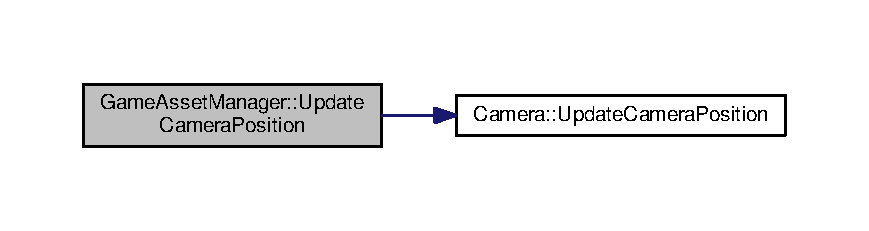
\includegraphics[width=350pt]{class_game_asset_manager_afbcf9d370cfefc67a696395f2cdf1a9b_cgraph}
\end{center}
\end{figure}




The documentation for this class was generated from the following files\+:\begin{DoxyCompactItemize}
\item 
src/\hyperlink{_game_asset_manager_8h}{Game\+Asset\+Manager.\+h}\item 
src/\hyperlink{_game_asset_manager_8cc}{Game\+Asset\+Manager.\+cc}\end{DoxyCompactItemize}

\hypertarget{class_game_world}{}\section{Game\+World Class Reference}
\label{class_game_world}\index{Game\+World@{Game\+World}}


{\ttfamily \#include $<$Game\+World.\+h$>$}

\subsection*{Public Member Functions}
\begin{DoxyCompactItemize}
\item 
\hyperlink{class_game_world_a681994123c12833d43c957d6cfb33765}{Game\+World} ()
\item 
void \hyperlink{class_game_world_a275418607d8286979b276f165ad5876b}{Draw} ()
\begin{DoxyCompactList}\small\item\em \char`\"{}\+Draw()\char`\"{} will draw the entire world. \end{DoxyCompactList}\item 
void \hyperlink{class_game_world_aa934714929b8b3bcf322f1ec4695d75b}{Update\+Camera\+Position} (\hyperlink{common_8h_a080a822f0093973313bd644e517a5090}{Input}, int mouse\+X, int mouse\+Y)
\end{DoxyCompactItemize}


\subsection{Detailed Description}
\hyperlink{class_game_world}{Game\+World} allows us to separate the management of the game world from the nuts and bolts of game loop initialisation. The \hyperlink{class_game_world}{Game\+World} currently has a very simplified scene graph consisiting of a single \hyperlink{class_game_asset_manager}{Game\+Asset\+Manager}. 

\subsection{Constructor \& Destructor Documentation}
\hypertarget{class_game_world_a681994123c12833d43c957d6cfb33765}{}\index{Game\+World@{Game\+World}!Game\+World@{Game\+World}}
\index{Game\+World@{Game\+World}!Game\+World@{Game\+World}}
\subsubsection[{Game\+World()}]{\setlength{\rightskip}{0pt plus 5cm}Game\+World\+::\+Game\+World (
\begin{DoxyParamCaption}
{}
\end{DoxyParamCaption}
)\hspace{0.3cm}{\ttfamily [explicit]}}\label{class_game_world_a681994123c12833d43c957d6cfb33765}
Cube spawning with Array Using a 2\+D array to spawn multiple voxels 1 -\/ Floor piece 2 -\/ Floor piece and cube 3 -\/ Floor piece and pyramid

Spawning Floor floor is spawned with; The values in the array above act like coordinate points. Y is a constant as the floor is one flat plane Z is determined by the Y value Add\+Asset Layout This adds the asset to the game asset manager which draws it to the screen asset\+\_\+manager-\/$>$Add\+Asset(make\+\_\+shared$<$\+Cube\+Asset$>$(\+Spawn, Translate, Animate\+To, Bool)

Spawning Cubes Spawns floor asset and a Cube asset

Spawning Pyramids Spawns floor asset and a Pyramid asset above it

\subsection{Member Function Documentation}
\hypertarget{class_game_world_a275418607d8286979b276f165ad5876b}{}\index{Game\+World@{Game\+World}!Draw@{Draw}}
\index{Draw@{Draw}!Game\+World@{Game\+World}}
\subsubsection[{Draw()}]{\setlength{\rightskip}{0pt plus 5cm}void Game\+World\+::\+Draw (
\begin{DoxyParamCaption}
{}
\end{DoxyParamCaption}
)}\label{class_game_world_a275418607d8286979b276f165ad5876b}


\char`\"{}\+Draw()\char`\"{} will draw the entire world. 

\hypertarget{class_game_world_aa934714929b8b3bcf322f1ec4695d75b}{}\index{Game\+World@{Game\+World}!Update\+Camera\+Position@{Update\+Camera\+Position}}
\index{Update\+Camera\+Position@{Update\+Camera\+Position}!Game\+World@{Game\+World}}
\subsubsection[{Update\+Camera\+Position(\+Input, int mouse\+X, int mouse\+Y)}]{\setlength{\rightskip}{0pt plus 5cm}void Game\+World\+::\+Update\+Camera\+Position (
\begin{DoxyParamCaption}
\item[{{\bf Input}}]{input\+\_\+direction, }
\item[{int}]{mouse\+X, }
\item[{int}]{mouse\+Y}
\end{DoxyParamCaption}
)}\label{class_game_world_aa934714929b8b3bcf322f1ec4695d75b}


The documentation for this class was generated from the following files\+:\begin{DoxyCompactItemize}
\item 
src/\hyperlink{_game_world_8h}{Game\+World.\+h}\item 
src/\hyperlink{_game_world_8cc}{Game\+World.\+cc}\end{DoxyCompactItemize}

\hypertarget{class_pyramid_asset}{}\section{Pyramid\+Asset Class Reference}
\label{class_pyramid_asset}\index{Pyramid\+Asset@{Pyramid\+Asset}}


{\ttfamily \#include $<$Pyramid\+Asset.\+h$>$}



Inheritance diagram for Pyramid\+Asset\+:
\nopagebreak
\begin{figure}[H]
\begin{center}
\leavevmode
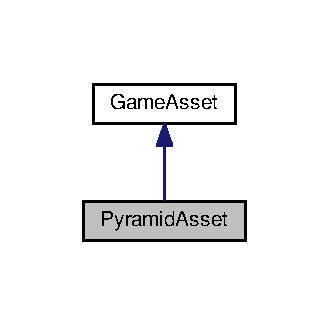
\includegraphics[width=158pt]{class_pyramid_asset__inherit__graph}
\end{center}
\end{figure}


Collaboration diagram for Pyramid\+Asset\+:
\nopagebreak
\begin{figure}[H]
\begin{center}
\leavevmode
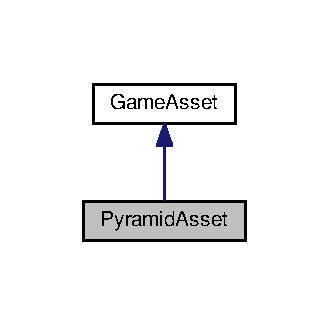
\includegraphics[width=158pt]{class_pyramid_asset__coll__graph}
\end{center}
\end{figure}
\subsection*{Public Member Functions}
\begin{DoxyCompactItemize}
\item 
\hyperlink{class_pyramid_asset_a5588f0b34bf4c71dc0ffe86ed5111b04}{Pyramid\+Asset} (glm\+::vec3 Spawn, glm\+::vec3 xyz\+Pos, glm\+::vec3 xyz\+Translation, bool xyz\+Tbool)
\item 
\hyperlink{class_pyramid_asset_afb388a196f43a3808b2d4f6fdb89ee84}{$\sim$\+Pyramid\+Asset} ()
\item 
virtual void \hyperlink{class_pyramid_asset_aaea45da4956d79ec9ab96e9d0ccef3fe}{Draw} (G\+Luint)
\end{DoxyCompactItemize}


\subsection{Constructor \& Destructor Documentation}
\hypertarget{class_pyramid_asset_a5588f0b34bf4c71dc0ffe86ed5111b04}{}\index{Pyramid\+Asset@{Pyramid\+Asset}!Pyramid\+Asset@{Pyramid\+Asset}}
\index{Pyramid\+Asset@{Pyramid\+Asset}!Pyramid\+Asset@{Pyramid\+Asset}}
\subsubsection[{Pyramid\+Asset(glm\+::vec3 Spawn, glm\+::vec3 xyz\+Pos, glm\+::vec3 xyz\+Translation, bool xyz\+Tbool)}]{\setlength{\rightskip}{0pt plus 5cm}Pyramid\+Asset\+::\+Pyramid\+Asset (
\begin{DoxyParamCaption}
\item[{glm\+::vec3}]{Spawn, }
\item[{glm\+::vec3}]{xyz\+Pos, }
\item[{glm\+::vec3}]{xyz\+Translation, }
\item[{bool}]{xyz\+Tbool}
\end{DoxyParamCaption}
)}\label{class_pyramid_asset_a5588f0b34bf4c71dc0ffe86ed5111b04}
Pyramid Creation models coordinates, origin dependant on xyz variables. vertex buffer models coordinates, for the triangles. colour buffer models the colour of the object triangles. element buffer creates the cube using 6 triangles.\hypertarget{class_pyramid_asset_afb388a196f43a3808b2d4f6fdb89ee84}{}\index{Pyramid\+Asset@{Pyramid\+Asset}!````~Pyramid\+Asset@{$\sim$\+Pyramid\+Asset}}
\index{````~Pyramid\+Asset@{$\sim$\+Pyramid\+Asset}!Pyramid\+Asset@{Pyramid\+Asset}}
\subsubsection[{$\sim$\+Pyramid\+Asset()}]{\setlength{\rightskip}{0pt plus 5cm}Pyramid\+Asset\+::$\sim$\+Pyramid\+Asset (
\begin{DoxyParamCaption}
{}
\end{DoxyParamCaption}
)}\label{class_pyramid_asset_afb388a196f43a3808b2d4f6fdb89ee84}


\subsection{Member Function Documentation}
\hypertarget{class_pyramid_asset_aaea45da4956d79ec9ab96e9d0ccef3fe}{}\index{Pyramid\+Asset@{Pyramid\+Asset}!Draw@{Draw}}
\index{Draw@{Draw}!Pyramid\+Asset@{Pyramid\+Asset}}
\subsubsection[{Draw(\+G\+Luint)}]{\setlength{\rightskip}{0pt plus 5cm}void Pyramid\+Asset\+::\+Draw (
\begin{DoxyParamCaption}
\item[{G\+Luint}]{program\+\_\+token}
\end{DoxyParamCaption}
)\hspace{0.3cm}{\ttfamily [virtual]}}\label{class_pyramid_asset_aaea45da4956d79ec9ab96e9d0ccef3fe}
use the previously transferred buffer as the vertex array. This way we transfer the buffer once -- at construction -- not on every frame.

repeated buffer array for color buffer

Implements \hyperlink{class_game_asset_a961aa51ca0a9961fc584c0b5d5431300}{Game\+Asset}.



The documentation for this class was generated from the following files\+:\begin{DoxyCompactItemize}
\item 
src/\hyperlink{_pyramid_asset_8h}{Pyramid\+Asset.\+h}\item 
src/\hyperlink{_pyramid_asset_8cc}{Pyramid\+Asset.\+cc}\end{DoxyCompactItemize}

\hypertarget{class_python_b}{}\section{Python\+B Class Reference}
\label{class_python_b}\index{Python\+B@{Python\+B}}


{\ttfamily \#include $<$Python\+B.\+h$>$}

\subsection*{Public Member Functions}
\begin{DoxyCompactItemize}
\item 
\hyperlink{class_python_b_a4ad68817aaed1c8ea4350935c16ad2c1}{Python\+B} ()
\end{DoxyCompactItemize}
\subsection*{Public Attributes}
\begin{DoxyCompactItemize}
\item 
tuple \hyperlink{class_python_b_a178da078caf1b800a95543460c7a12f5}{Start} = liblink.\+Game()
\end{DoxyCompactItemize}


\subsection{Constructor \& Destructor Documentation}
\hypertarget{class_python_b_a4ad68817aaed1c8ea4350935c16ad2c1}{}\index{Python\+B@{Python\+B}!Python\+B@{Python\+B}}
\index{Python\+B@{Python\+B}!Python\+B@{Python\+B}}
\subsubsection[{Python\+B()}]{\setlength{\rightskip}{0pt plus 5cm}Python\+B\+::\+Python\+B (
\begin{DoxyParamCaption}
{}
\end{DoxyParamCaption}
)}\label{class_python_b_a4ad68817aaed1c8ea4350935c16ad2c1}


\subsection{Member Data Documentation}
\hypertarget{class_python_b_a178da078caf1b800a95543460c7a12f5}{}\index{Python\+B@{Python\+B}!Start@{Start}}
\index{Start@{Start}!Python\+B@{Python\+B}}
\subsubsection[{Start}]{\setlength{\rightskip}{0pt plus 5cm}tuple Python\+B.\+Start = liblink.\+Game()}\label{class_python_b_a178da078caf1b800a95543460c7a12f5}


The documentation for this class was generated from the following files\+:\begin{DoxyCompactItemize}
\item 
src/\hyperlink{_python_b_8h}{Python\+B.\+h}\item 
src/\hyperlink{_python_b_8py}{Python\+B.\+py}\item 
src/\hyperlink{_python_b_8cc}{Python\+B.\+cc}\end{DoxyCompactItemize}

\hypertarget{struct_s_d_l_window_deleter}{}\section{S\+D\+L\+Window\+Deleter Struct Reference}
\label{struct_s_d_l_window_deleter}\index{S\+D\+L\+Window\+Deleter@{S\+D\+L\+Window\+Deleter}}
\subsection*{Public Member Functions}
\begin{DoxyCompactItemize}
\item 
void \hyperlink{struct_s_d_l_window_deleter_a2aedcc99c3756ae090c38badabeb10b1}{operator()} (S\+D\+L\+\_\+\+Window $\ast$window)
\end{DoxyCompactItemize}


\subsection{Member Function Documentation}
\hypertarget{struct_s_d_l_window_deleter_a2aedcc99c3756ae090c38badabeb10b1}{}\index{S\+D\+L\+Window\+Deleter@{S\+D\+L\+Window\+Deleter}!operator()@{operator()}}
\index{operator()@{operator()}!S\+D\+L\+Window\+Deleter@{S\+D\+L\+Window\+Deleter}}
\subsubsection[{operator()(\+S\+D\+L\+\_\+\+Window $\ast$window)}]{\setlength{\rightskip}{0pt plus 5cm}void S\+D\+L\+Window\+Deleter\+::operator() (
\begin{DoxyParamCaption}
\item[{S\+D\+L\+\_\+\+Window $\ast$}]{window}
\end{DoxyParamCaption}
)\hspace{0.3cm}{\ttfamily [inline]}}\label{struct_s_d_l_window_deleter_a2aedcc99c3756ae090c38badabeb10b1}


The documentation for this struct was generated from the following file\+:\begin{DoxyCompactItemize}
\item 
src/\hyperlink{_game_8cc}{Game.\+cc}\end{DoxyCompactItemize}

\chapter{File Documentation}
\hypertarget{_bounding_box_8cc}{}\section{src/\+Bounding\+Box.cc File Reference}
\label{_bounding_box_8cc}\index{src/\+Bounding\+Box.\+cc@{src/\+Bounding\+Box.\+cc}}
{\ttfamily \#include \char`\"{}Bounding\+Box.\+h\char`\"{}}\\*
Include dependency graph for Bounding\+Box.\+cc\+:\nopagebreak
\begin{figure}[H]
\begin{center}
\leavevmode
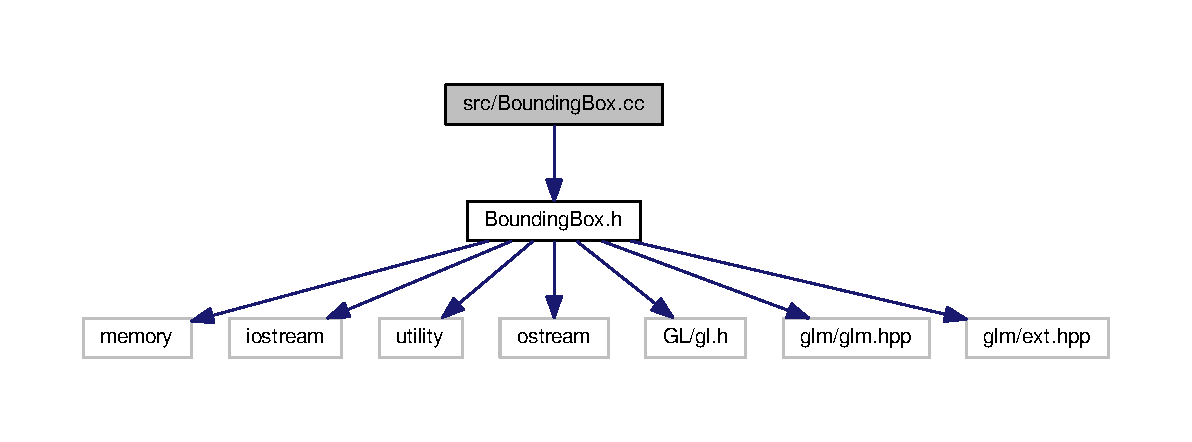
\includegraphics[width=350pt]{_bounding_box_8cc__incl}
\end{center}
\end{figure}

\hypertarget{_bounding_box_8h}{}\section{src/\+Bounding\+Box.h File Reference}
\label{_bounding_box_8h}\index{src/\+Bounding\+Box.\+h@{src/\+Bounding\+Box.\+h}}
{\ttfamily \#include $<$memory$>$}\\*
{\ttfamily \#include $<$iostream$>$}\\*
{\ttfamily \#include $<$utility$>$}\\*
{\ttfamily \#include $<$ostream$>$}\\*
{\ttfamily \#include $<$G\+L/gl.\+h$>$}\\*
{\ttfamily \#include $<$glm/glm.\+hpp$>$}\\*
{\ttfamily \#include $<$glm/ext.\+hpp$>$}\\*
Include dependency graph for Bounding\+Box.\+h\+:\nopagebreak
\begin{figure}[H]
\begin{center}
\leavevmode
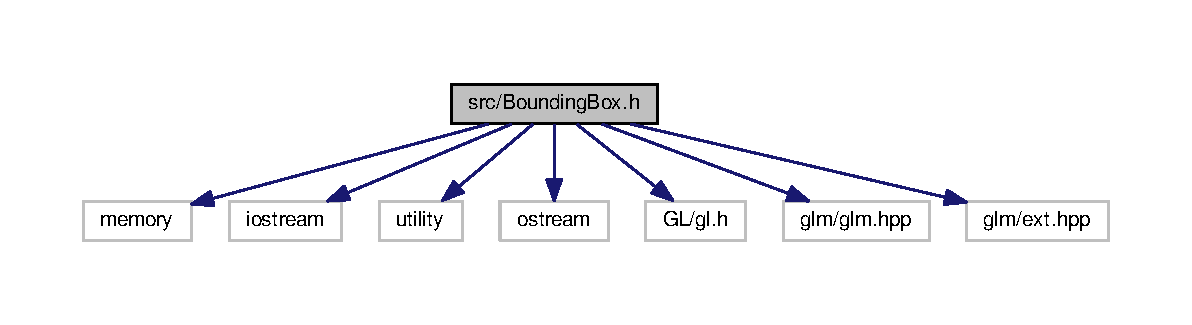
\includegraphics[width=350pt]{_bounding_box_8h__incl}
\end{center}
\end{figure}
This graph shows which files directly or indirectly include this file\+:\nopagebreak
\begin{figure}[H]
\begin{center}
\leavevmode
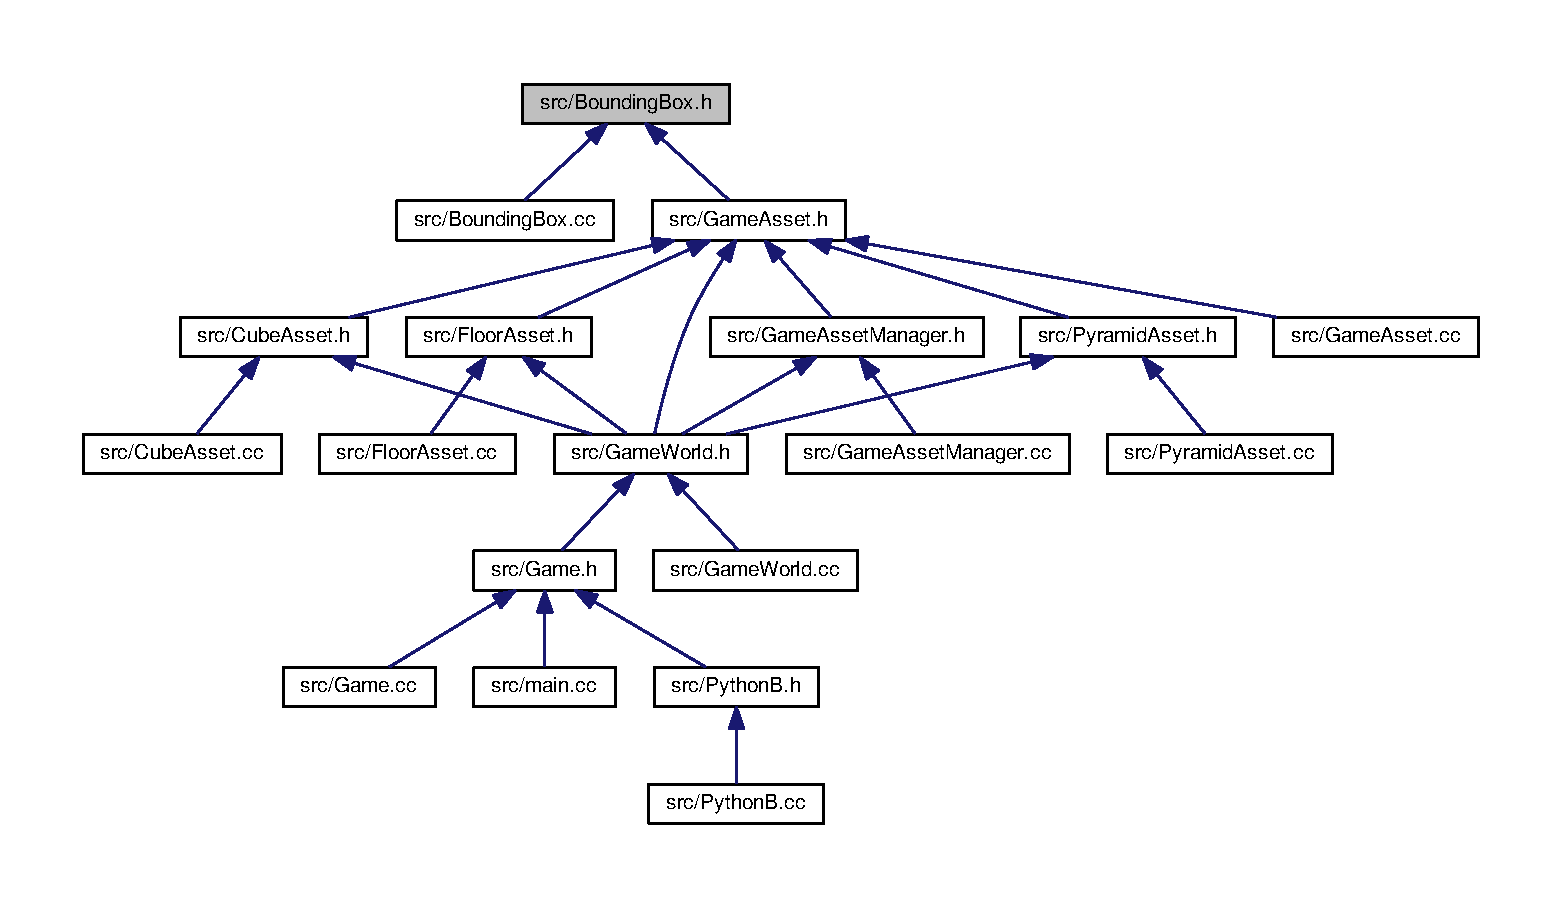
\includegraphics[width=350pt]{_bounding_box_8h__dep__incl}
\end{center}
\end{figure}
\subsection*{Classes}
\begin{DoxyCompactItemize}
\item 
class \hyperlink{class_bounding_box}{Bounding\+Box}
\end{DoxyCompactItemize}

\hypertarget{_camera_8cc}{}\section{src/\+Camera.cc File Reference}
\label{_camera_8cc}\index{src/\+Camera.\+cc@{src/\+Camera.\+cc}}
{\ttfamily \#include \char`\"{}Camera.\+h\char`\"{}}\\*
{\ttfamily \#include $<$glm/ext.\+hpp$>$}\\*
Include dependency graph for Camera.\+cc\+:\nopagebreak
\begin{figure}[H]
\begin{center}
\leavevmode
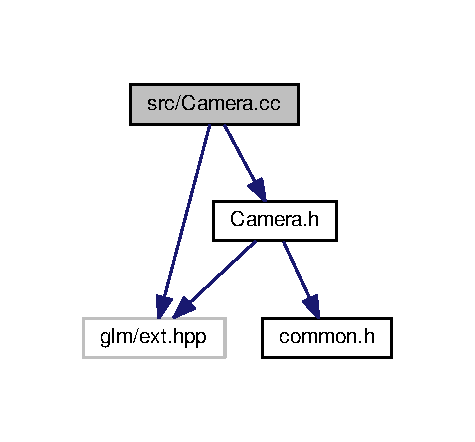
\includegraphics[width=228pt]{_camera_8cc__incl}
\end{center}
\end{figure}

\hypertarget{_camera_8h}{}\section{src/\+Camera.h File Reference}
\label{_camera_8h}\index{src/\+Camera.\+h@{src/\+Camera.\+h}}
{\ttfamily \#include $<$glm/ext.\+hpp$>$}\\*
{\ttfamily \#include \char`\"{}common.\+h\char`\"{}}\\*
Include dependency graph for Camera.\+h\+:\nopagebreak
\begin{figure}[H]
\begin{center}
\leavevmode
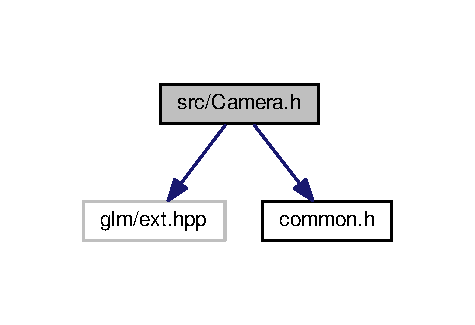
\includegraphics[width=228pt]{_camera_8h__incl}
\end{center}
\end{figure}
This graph shows which files directly or indirectly include this file\+:\nopagebreak
\begin{figure}[H]
\begin{center}
\leavevmode
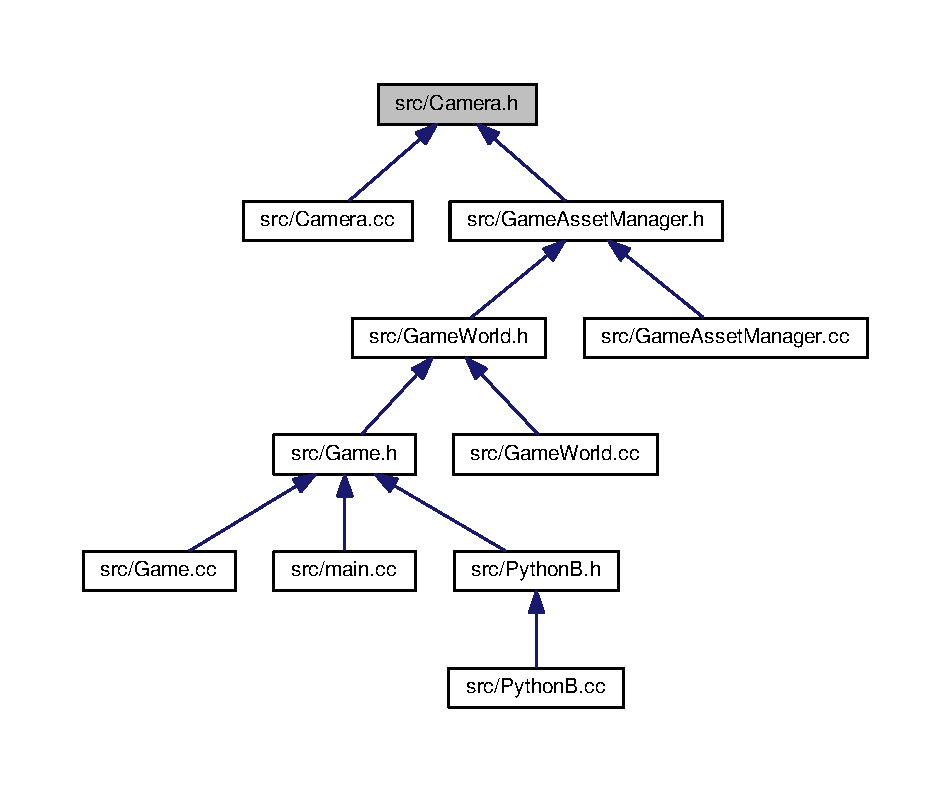
\includegraphics[width=350pt]{_camera_8h__dep__incl}
\end{center}
\end{figure}
\subsection*{Classes}
\begin{DoxyCompactItemize}
\item 
class \hyperlink{class_camera}{Camera}
\end{DoxyCompactItemize}

\hypertarget{common_8h}{}\section{src/common.h File Reference}
\label{common_8h}\index{src/common.\+h@{src/common.\+h}}
This graph shows which files directly or indirectly include this file\+:
\nopagebreak
\begin{figure}[H]
\begin{center}
\leavevmode
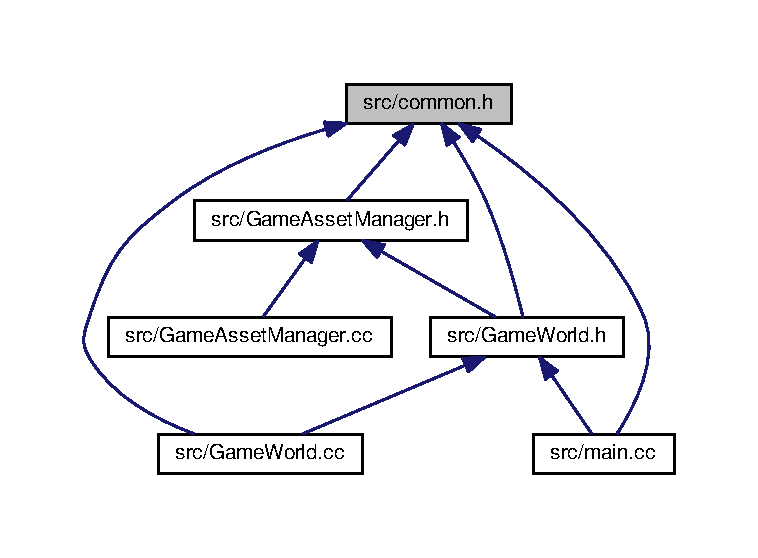
\includegraphics[width=350pt]{common_8h__dep__incl}
\end{center}
\end{figure}
\subsection*{Enumerations}
\begin{DoxyCompactItemize}
\item 
enum \hyperlink{common_8h_add86e7c88dd109abea3f708b422f31f0}{Application\+Mode} \{ \hyperlink{common_8h_add86e7c88dd109abea3f708b422f31f0a25f73324dc93d9024c0c75b4e6815335}{T\+R\+A\+N\+S\+F\+O\+R\+M}, 
\hyperlink{common_8h_add86e7c88dd109abea3f708b422f31f0a3dcfe0046eb5876e287dbf0914819b16}{R\+O\+T\+A\+T\+E}, 
\hyperlink{common_8h_add86e7c88dd109abea3f708b422f31f0a593be05a10070b4e7e0856e20590eaaf}{S\+C\+A\+L\+E}
 \}\begin{DoxyCompactList}\small\item\em Application\+Mode denotes the global state of the application. \end{DoxyCompactList}
\end{DoxyCompactItemize}


\subsection{Enumeration Type Documentation}
\hypertarget{common_8h_add86e7c88dd109abea3f708b422f31f0}{}\index{common.\+h@{common.\+h}!Application\+Mode@{Application\+Mode}}
\index{Application\+Mode@{Application\+Mode}!common.\+h@{common.\+h}}
\subsubsection[{Application\+Mode}]{\setlength{\rightskip}{0pt plus 5cm}enum {\bf Application\+Mode}}\label{common_8h_add86e7c88dd109abea3f708b422f31f0}


Application\+Mode denotes the global state of the application. 

There are three global states for this application\+:
\begin{DoxyEnumerate}
\item Transform -- load the correct shaders to do a transformation of a simple asset.
\item Rotate -- load the correct shader to rotate a simple asset.
\item Scale -- load the correct shader to scale a simple asset. 
\end{DoxyEnumerate}\begin{Desc}
\item[Enumerator]\par
\begin{description}
\index{T\+R\+A\+N\+S\+F\+O\+R\+M@{T\+R\+A\+N\+S\+F\+O\+R\+M}!common.\+h@{common.\+h}}\index{common.\+h@{common.\+h}!T\+R\+A\+N\+S\+F\+O\+R\+M@{T\+R\+A\+N\+S\+F\+O\+R\+M}}\item[{\em 
\hypertarget{common_8h_add86e7c88dd109abea3f708b422f31f0a25f73324dc93d9024c0c75b4e6815335}{}T\+R\+A\+N\+S\+F\+O\+R\+M\label{common_8h_add86e7c88dd109abea3f708b422f31f0a25f73324dc93d9024c0c75b4e6815335}
}]\index{R\+O\+T\+A\+T\+E@{R\+O\+T\+A\+T\+E}!common.\+h@{common.\+h}}\index{common.\+h@{common.\+h}!R\+O\+T\+A\+T\+E@{R\+O\+T\+A\+T\+E}}\item[{\em 
\hypertarget{common_8h_add86e7c88dd109abea3f708b422f31f0a3dcfe0046eb5876e287dbf0914819b16}{}R\+O\+T\+A\+T\+E\label{common_8h_add86e7c88dd109abea3f708b422f31f0a3dcfe0046eb5876e287dbf0914819b16}
}]\index{S\+C\+A\+L\+E@{S\+C\+A\+L\+E}!common.\+h@{common.\+h}}\index{common.\+h@{common.\+h}!S\+C\+A\+L\+E@{S\+C\+A\+L\+E}}\item[{\em 
\hypertarget{common_8h_add86e7c88dd109abea3f708b422f31f0a593be05a10070b4e7e0856e20590eaaf}{}S\+C\+A\+L\+E\label{common_8h_add86e7c88dd109abea3f708b422f31f0a593be05a10070b4e7e0856e20590eaaf}
}]\end{description}
\end{Desc}

\begin{DoxyCode}
12 \{\hyperlink{common_8h_add86e7c88dd109abea3f708b422f31f0a25f73324dc93d9024c0c75b4e6815335}{TRANSFORM}, \hyperlink{common_8h_add86e7c88dd109abea3f708b422f31f0a3dcfe0046eb5876e287dbf0914819b16}{ROTATE}, \hyperlink{common_8h_add86e7c88dd109abea3f708b422f31f0a593be05a10070b4e7e0856e20590eaaf}{SCALE}\};
\end{DoxyCode}

\hypertarget{_cube_asset_8cc}{}\section{src/\+Cube\+Asset.cc File Reference}
\label{_cube_asset_8cc}\index{src/\+Cube\+Asset.\+cc@{src/\+Cube\+Asset.\+cc}}
{\ttfamily \#include \char`\"{}Cube\+Asset.\+h\char`\"{}}\\*
Include dependency graph for Cube\+Asset.\+cc\+:
\nopagebreak
\begin{figure}[H]
\begin{center}
\leavevmode
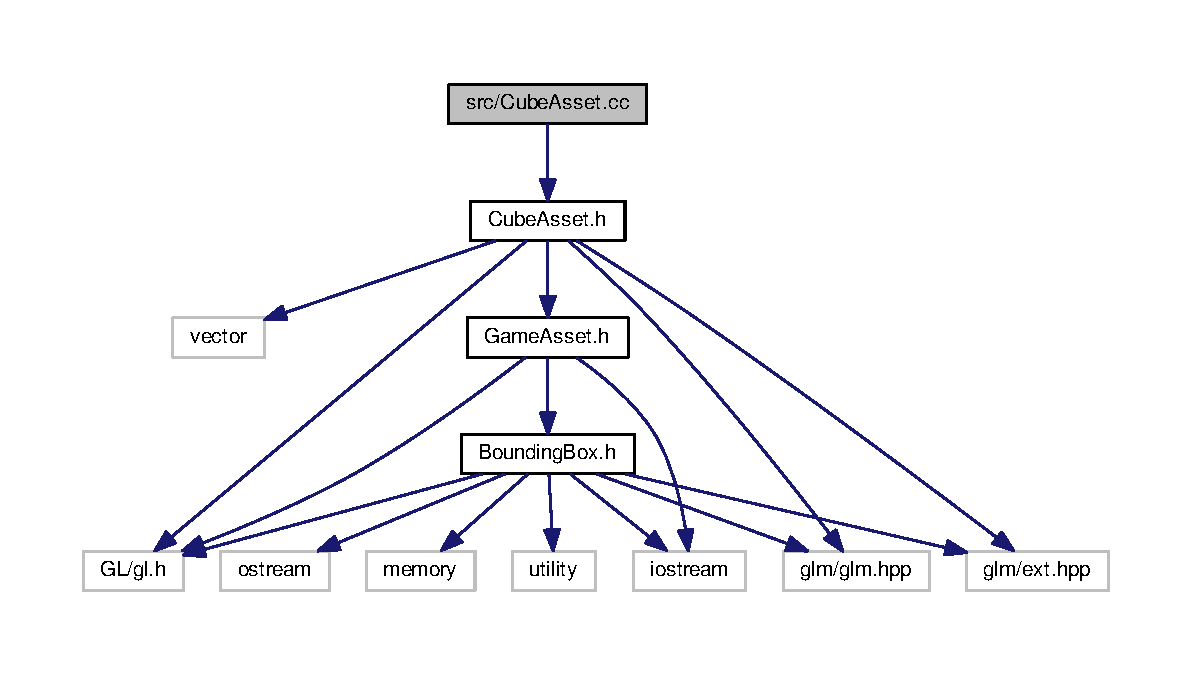
\includegraphics[width=350pt]{_cube_asset_8cc__incl}
\end{center}
\end{figure}
\subsection*{Macros}
\begin{DoxyCompactItemize}
\item 
\#define \hyperlink{_cube_asset_8cc_a75f201b0e53e68726854997957322b8d}{check\+G\+L\+Error}()
\end{DoxyCompactItemize}


\subsection{Macro Definition Documentation}
\hypertarget{_cube_asset_8cc_a75f201b0e53e68726854997957322b8d}{}\index{Cube\+Asset.\+cc@{Cube\+Asset.\+cc}!check\+G\+L\+Error@{check\+G\+L\+Error}}
\index{check\+G\+L\+Error@{check\+G\+L\+Error}!Cube\+Asset.\+cc@{Cube\+Asset.\+cc}}
\subsubsection[{check\+G\+L\+Error}]{\setlength{\rightskip}{0pt plus 5cm}\#define check\+G\+L\+Error(
\begin{DoxyParamCaption}
{}
\end{DoxyParamCaption}
)}\label{_cube_asset_8cc_a75f201b0e53e68726854997957322b8d}

\hypertarget{_cube_asset_8h}{}\section{src/\+Cube\+Asset.h File Reference}
\label{_cube_asset_8h}\index{src/\+Cube\+Asset.\+h@{src/\+Cube\+Asset.\+h}}
{\ttfamily \#include $<$vector$>$}\\*
{\ttfamily \#include $<$G\+L/gl.\+h$>$}\\*
{\ttfamily \#include $<$glm/glm.\+hpp$>$}\\*
{\ttfamily \#include $<$glm/ext.\+hpp$>$}\\*
{\ttfamily \#include \char`\"{}Game\+Asset.\+h\char`\"{}}\\*
Include dependency graph for Cube\+Asset.\+h\+:\nopagebreak
\begin{figure}[H]
\begin{center}
\leavevmode
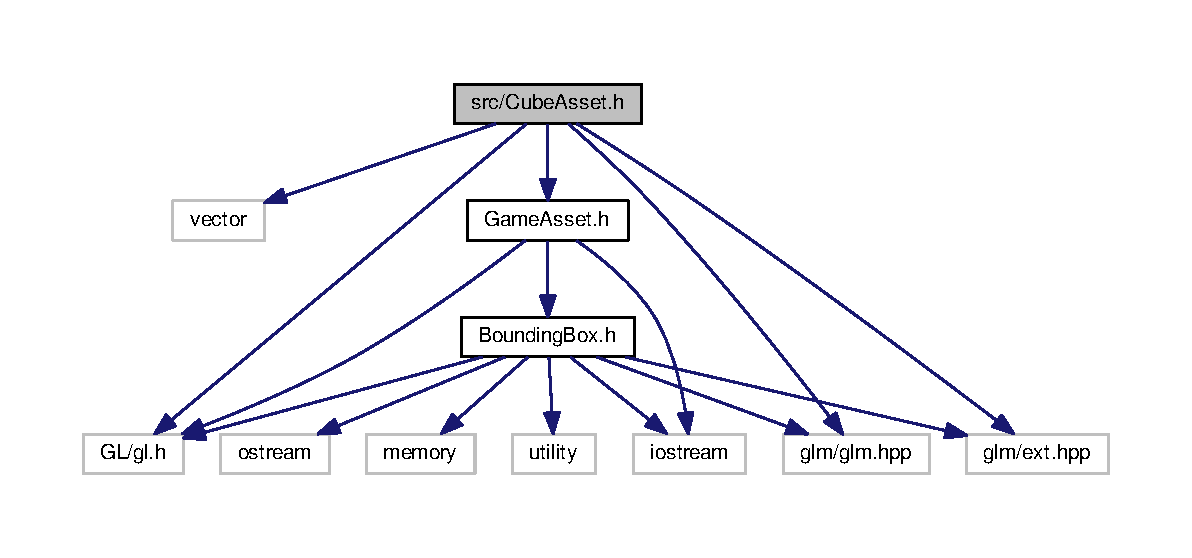
\includegraphics[width=350pt]{_cube_asset_8h__incl}
\end{center}
\end{figure}
This graph shows which files directly or indirectly include this file\+:\nopagebreak
\begin{figure}[H]
\begin{center}
\leavevmode
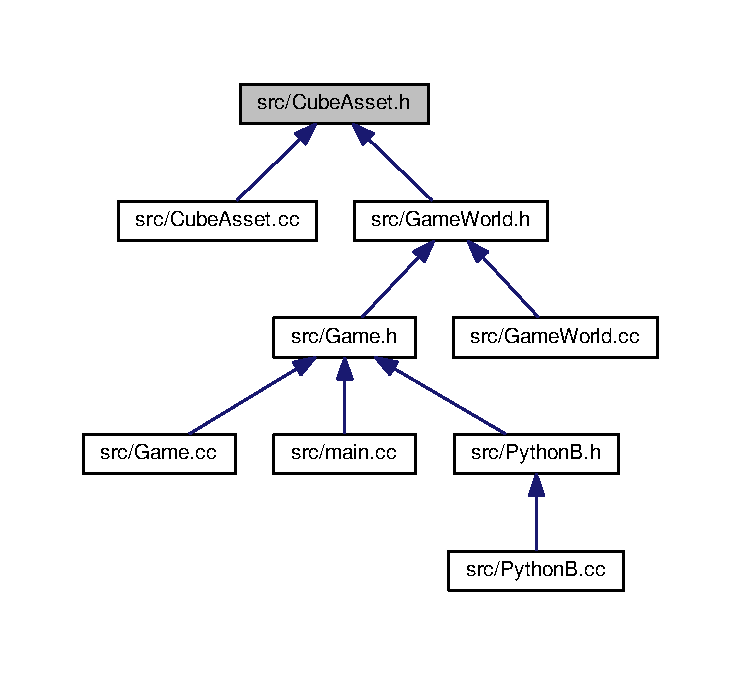
\includegraphics[width=350pt]{_cube_asset_8h__dep__incl}
\end{center}
\end{figure}
\subsection*{Classes}
\begin{DoxyCompactItemize}
\item 
class \hyperlink{class_cube_asset}{Cube\+Asset}
\end{DoxyCompactItemize}

\hypertarget{_floor_asset_8cc}{}\section{src/\+Floor\+Asset.cc File Reference}
\label{_floor_asset_8cc}\index{src/\+Floor\+Asset.\+cc@{src/\+Floor\+Asset.\+cc}}
{\ttfamily \#include \char`\"{}Floor\+Asset.\+h\char`\"{}}\\*
Include dependency graph for Floor\+Asset.\+cc\+:\nopagebreak
\begin{figure}[H]
\begin{center}
\leavevmode
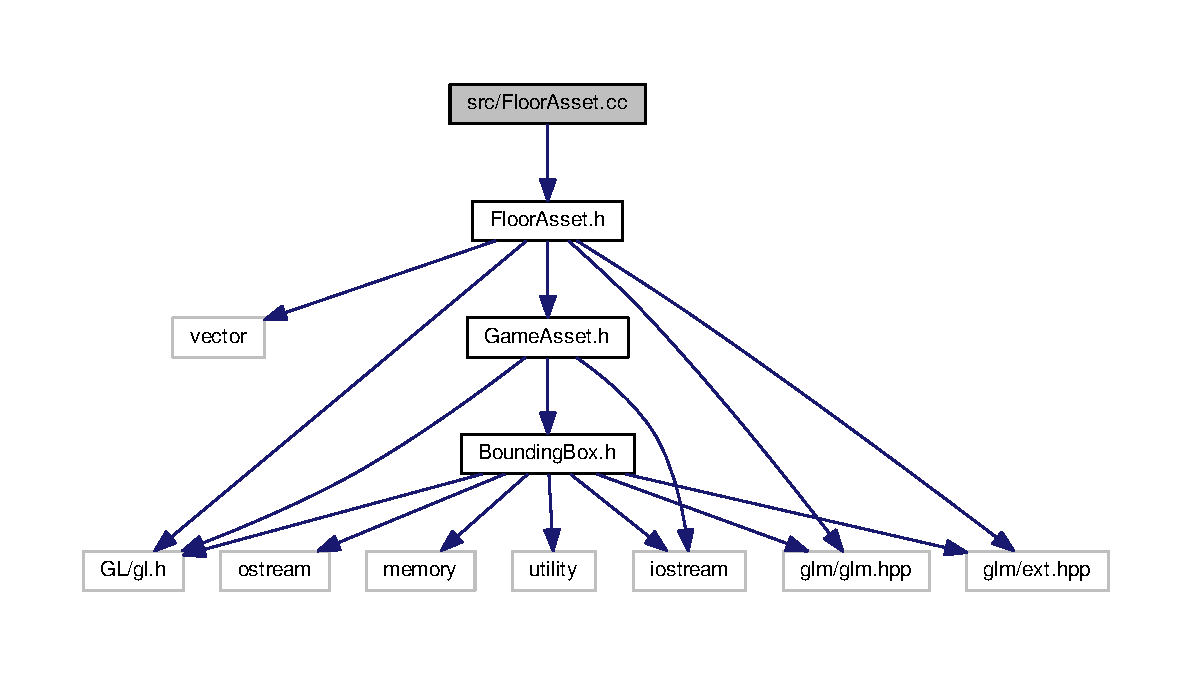
\includegraphics[width=350pt]{_floor_asset_8cc__incl}
\end{center}
\end{figure}
\subsection*{Macros}
\begin{DoxyCompactItemize}
\item 
\#define \hyperlink{_floor_asset_8cc_a75f201b0e53e68726854997957322b8d}{check\+G\+L\+Error}()
\end{DoxyCompactItemize}


\subsection{Macro Definition Documentation}
\hypertarget{_floor_asset_8cc_a75f201b0e53e68726854997957322b8d}{}\index{Floor\+Asset.\+cc@{Floor\+Asset.\+cc}!check\+G\+L\+Error@{check\+G\+L\+Error}}
\index{check\+G\+L\+Error@{check\+G\+L\+Error}!Floor\+Asset.\+cc@{Floor\+Asset.\+cc}}
\subsubsection[{check\+G\+L\+Error}]{\setlength{\rightskip}{0pt plus 5cm}\#define check\+G\+L\+Error(
\begin{DoxyParamCaption}
{}
\end{DoxyParamCaption}
)}\label{_floor_asset_8cc_a75f201b0e53e68726854997957322b8d}

\hypertarget{_floor_asset_8h}{}\section{src/\+Floor\+Asset.h File Reference}
\label{_floor_asset_8h}\index{src/\+Floor\+Asset.\+h@{src/\+Floor\+Asset.\+h}}
{\ttfamily \#include $<$vector$>$}\\*
{\ttfamily \#include $<$G\+L/gl.\+h$>$}\\*
{\ttfamily \#include $<$glm/glm.\+hpp$>$}\\*
{\ttfamily \#include $<$glm/ext.\+hpp$>$}\\*
{\ttfamily \#include \char`\"{}Game\+Asset.\+h\char`\"{}}\\*
Include dependency graph for Floor\+Asset.\+h\+:
\nopagebreak
\begin{figure}[H]
\begin{center}
\leavevmode
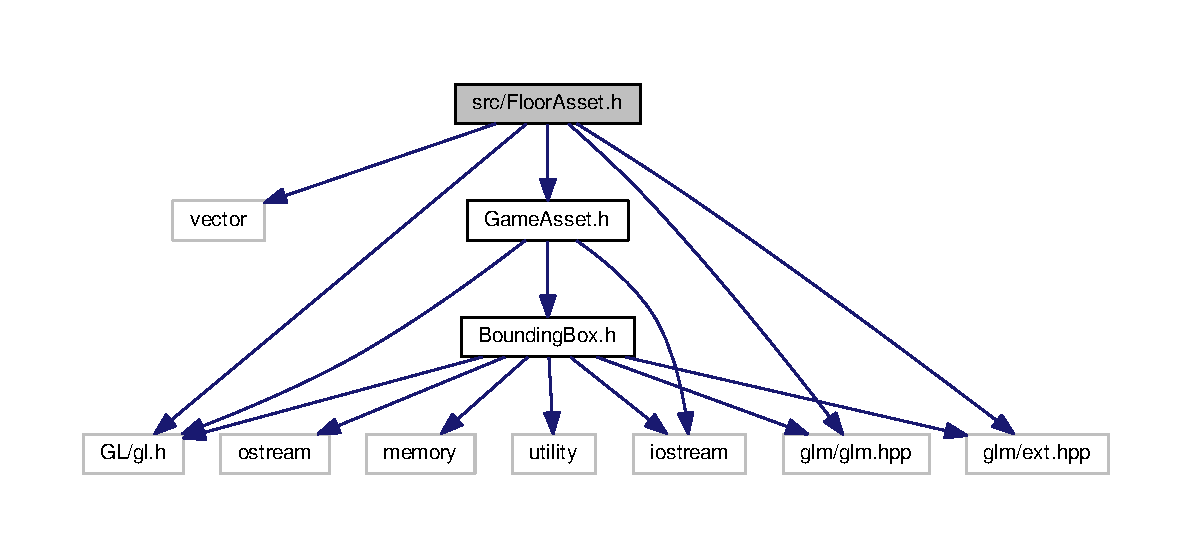
\includegraphics[width=350pt]{_floor_asset_8h__incl}
\end{center}
\end{figure}
This graph shows which files directly or indirectly include this file\+:
\nopagebreak
\begin{figure}[H]
\begin{center}
\leavevmode
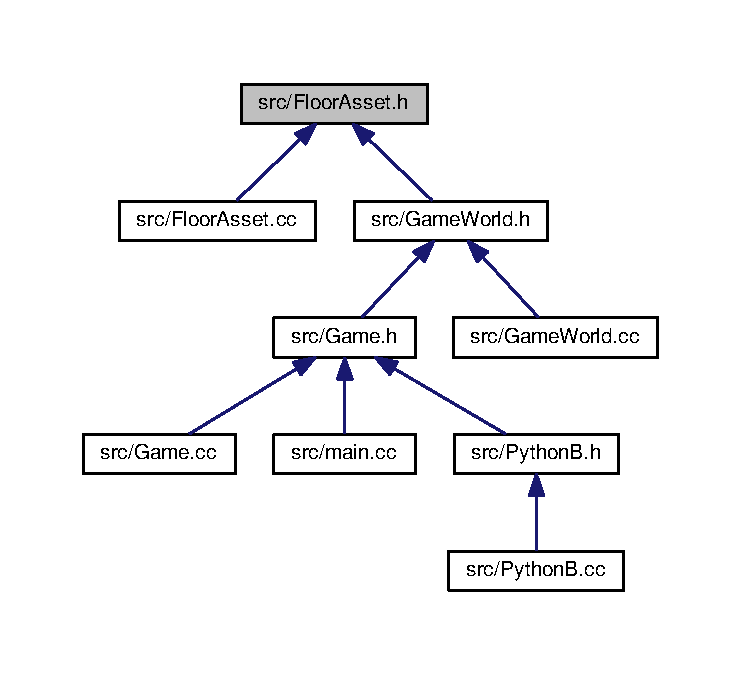
\includegraphics[width=350pt]{_floor_asset_8h__dep__incl}
\end{center}
\end{figure}
\subsection*{Classes}
\begin{DoxyCompactItemize}
\item 
class \hyperlink{class_floor_asset}{Floor\+Asset}
\end{DoxyCompactItemize}

\hypertarget{_game_8cc}{}\section{src/\+Game.cc File Reference}
\label{_game_8cc}\index{src/\+Game.\+cc@{src/\+Game.\+cc}}
{\ttfamily \#include $<$G\+L/glew.\+h$>$}\\*
{\ttfamily \#include $<$G\+L/gl.\+h$>$}\\*
{\ttfamily \#include $<$S\+D\+L2/\+S\+D\+L.\+h$>$}\\*
{\ttfamily \#include $<$iostream$>$}\\*
{\ttfamily \#include $<$memory$>$}\\*
{\ttfamily \#include $<$boost/program\+\_\+options.\+hpp$>$}\\*
{\ttfamily \#include \char`\"{}common.\+h\char`\"{}}\\*
{\ttfamily \#include \char`\"{}Game.\+h\char`\"{}}\\*
Include dependency graph for Game.\+cc\+:\nopagebreak
\begin{figure}[H]
\begin{center}
\leavevmode
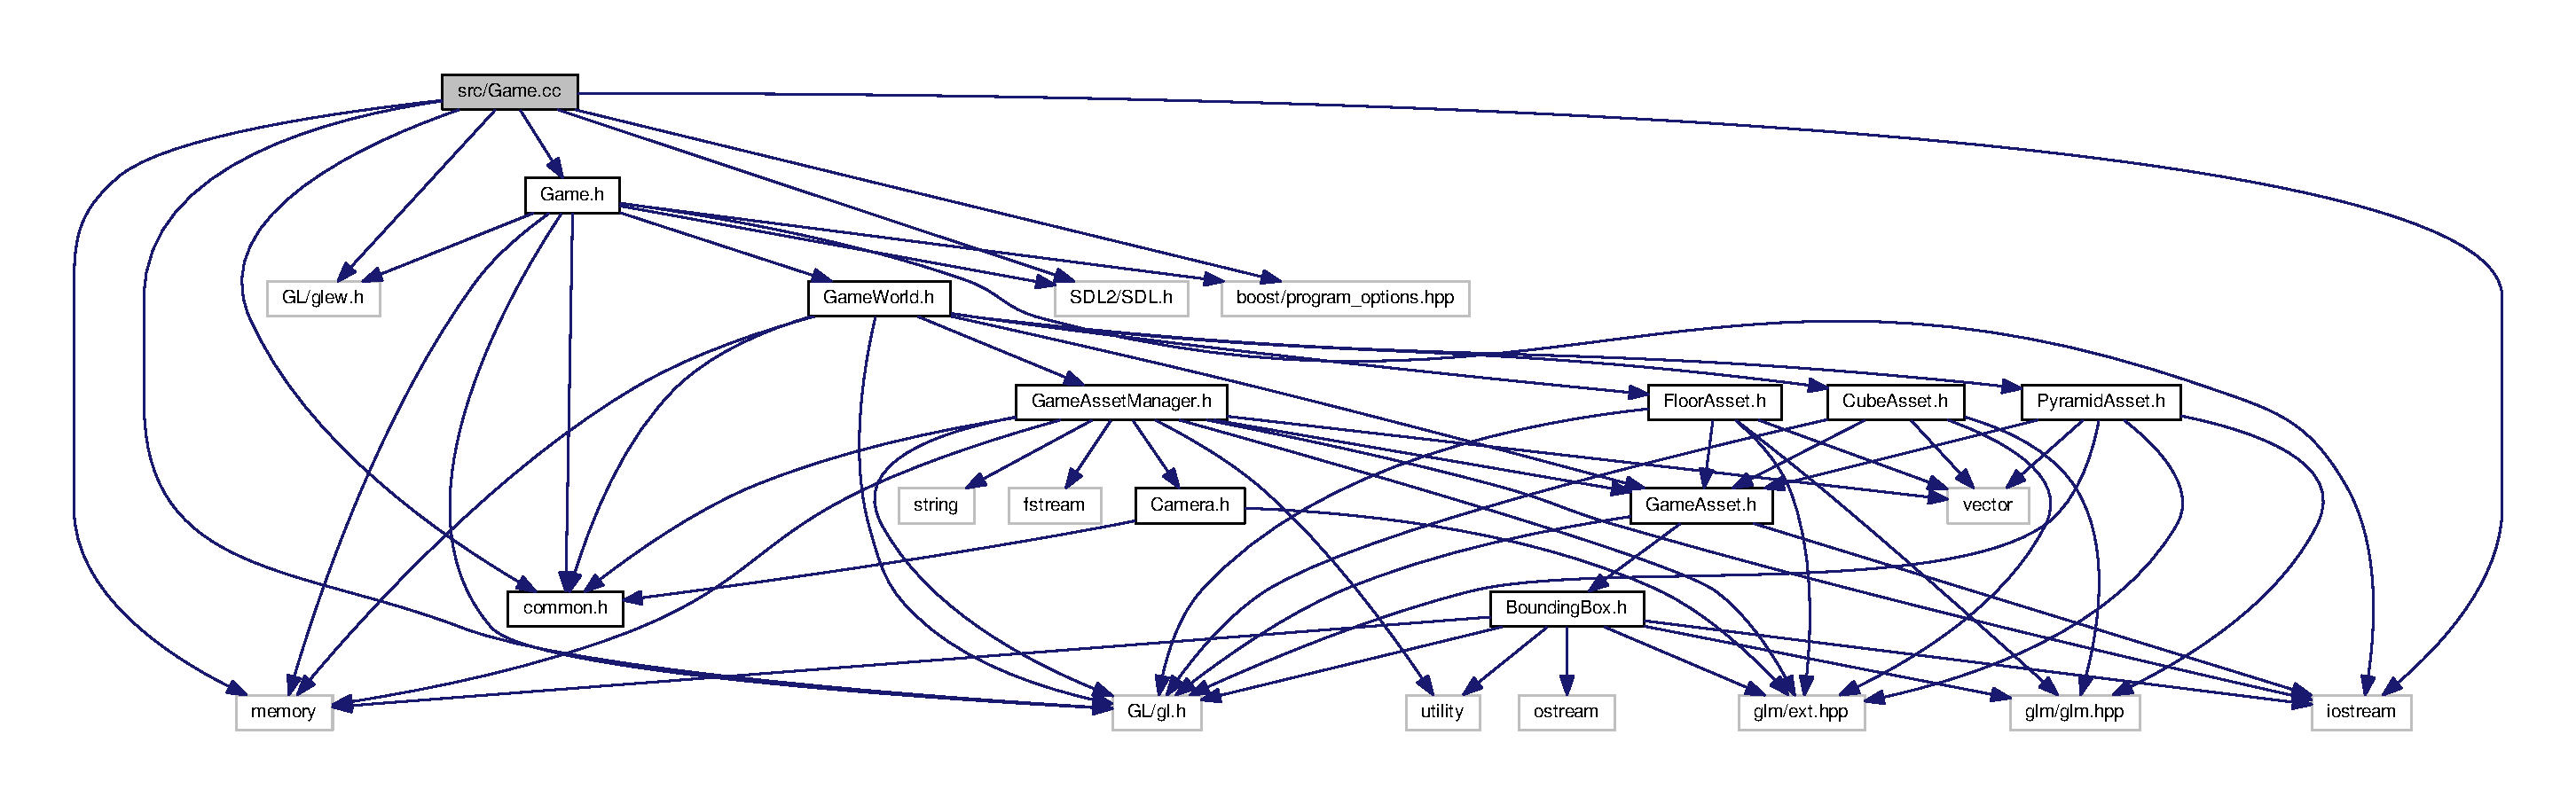
\includegraphics[width=350pt]{_game_8cc__incl}
\end{center}
\end{figure}
\subsection*{Classes}
\begin{DoxyCompactItemize}
\item 
struct \hyperlink{struct_s_d_l_window_deleter}{S\+D\+L\+Window\+Deleter}
\end{DoxyCompactItemize}
\subsection*{Macros}
\begin{DoxyCompactItemize}
\item 
\#define \hyperlink{_game_8cc_abcde84ea0ef5f934384e4620f092c85a}{G\+L\+E\+W\+\_\+\+S\+T\+A\+T\+I\+C}
\item 
\#define \hyperlink{_game_8cc_a6ff0ea1b288e03115f981ba31f96fade}{R\+U\+N\+\_\+\+G\+R\+A\+P\+H\+I\+C\+S\+\_\+\+D\+I\+S\+P\+L\+A\+Y}~0x00;
\end{DoxyCompactItemize}
\subsection*{Functions}
\begin{DoxyCompactItemize}
\item 
Uint32 \hyperlink{_game_8cc_a70eaa727262f633037c3f4b7d3ff24c2}{tick} (Uint32 interval, void $\ast$param)
\end{DoxyCompactItemize}


\subsection{Macro Definition Documentation}
\hypertarget{_game_8cc_abcde84ea0ef5f934384e4620f092c85a}{}\index{Game.\+cc@{Game.\+cc}!G\+L\+E\+W\+\_\+\+S\+T\+A\+T\+I\+C@{G\+L\+E\+W\+\_\+\+S\+T\+A\+T\+I\+C}}
\index{G\+L\+E\+W\+\_\+\+S\+T\+A\+T\+I\+C@{G\+L\+E\+W\+\_\+\+S\+T\+A\+T\+I\+C}!Game.\+cc@{Game.\+cc}}
\subsubsection[{G\+L\+E\+W\+\_\+\+S\+T\+A\+T\+I\+C}]{\setlength{\rightskip}{0pt plus 5cm}\#define G\+L\+E\+W\+\_\+\+S\+T\+A\+T\+I\+C}\label{_game_8cc_abcde84ea0ef5f934384e4620f092c85a}
\hypertarget{_game_8cc_a6ff0ea1b288e03115f981ba31f96fade}{}\index{Game.\+cc@{Game.\+cc}!R\+U\+N\+\_\+\+G\+R\+A\+P\+H\+I\+C\+S\+\_\+\+D\+I\+S\+P\+L\+A\+Y@{R\+U\+N\+\_\+\+G\+R\+A\+P\+H\+I\+C\+S\+\_\+\+D\+I\+S\+P\+L\+A\+Y}}
\index{R\+U\+N\+\_\+\+G\+R\+A\+P\+H\+I\+C\+S\+\_\+\+D\+I\+S\+P\+L\+A\+Y@{R\+U\+N\+\_\+\+G\+R\+A\+P\+H\+I\+C\+S\+\_\+\+D\+I\+S\+P\+L\+A\+Y}!Game.\+cc@{Game.\+cc}}
\subsubsection[{R\+U\+N\+\_\+\+G\+R\+A\+P\+H\+I\+C\+S\+\_\+\+D\+I\+S\+P\+L\+A\+Y}]{\setlength{\rightskip}{0pt plus 5cm}\#define R\+U\+N\+\_\+\+G\+R\+A\+P\+H\+I\+C\+S\+\_\+\+D\+I\+S\+P\+L\+A\+Y~0x00;}\label{_game_8cc_a6ff0ea1b288e03115f981ba31f96fade}


\subsection{Function Documentation}
\hypertarget{_game_8cc_a70eaa727262f633037c3f4b7d3ff24c2}{}\index{Game.\+cc@{Game.\+cc}!tick@{tick}}
\index{tick@{tick}!Game.\+cc@{Game.\+cc}}
\subsubsection[{tick(\+Uint32 interval, void $\ast$param)}]{\setlength{\rightskip}{0pt plus 5cm}Uint32 tick (
\begin{DoxyParamCaption}
\item[{Uint32}]{interval, }
\item[{void $\ast$}]{param}
\end{DoxyParamCaption}
)}\label{_game_8cc_a70eaa727262f633037c3f4b7d3ff24c2}
S\+D\+L timers run in separate threads. In the timer thread push an event onto the event queue. This event signifies to call display() from the thread in which the Open\+G\+L context was created. 

Here is the caller graph for this function\+:\nopagebreak
\begin{figure}[H]
\begin{center}
\leavevmode
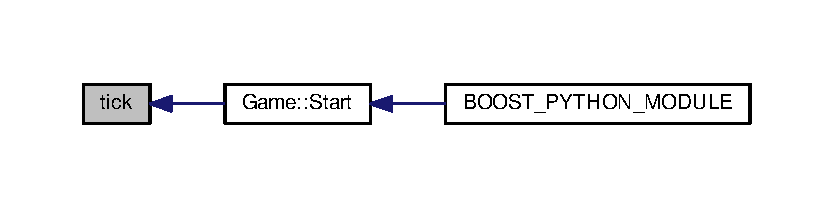
\includegraphics[width=350pt]{_game_8cc_a70eaa727262f633037c3f4b7d3ff24c2_icgraph}
\end{center}
\end{figure}



\hypertarget{_game_8h}{}\section{src/\+Game.h File Reference}
\label{_game_8h}\index{src/\+Game.\+h@{src/\+Game.\+h}}
{\ttfamily \#include $<$G\+L/glew.\+h$>$}\\*
{\ttfamily \#include $<$G\+L/gl.\+h$>$}\\*
{\ttfamily \#include $<$S\+D\+L2/\+S\+D\+L.\+h$>$}\\*
{\ttfamily \#include $<$iostream$>$}\\*
{\ttfamily \#include $<$memory$>$}\\*
{\ttfamily \#include $<$boost/program\+\_\+options.\+hpp$>$}\\*
{\ttfamily \#include \char`\"{}common.\+h\char`\"{}}\\*
{\ttfamily \#include \char`\"{}Game\+World.\+h\char`\"{}}\\*
Include dependency graph for Game.\+h\+:\nopagebreak
\begin{figure}[H]
\begin{center}
\leavevmode
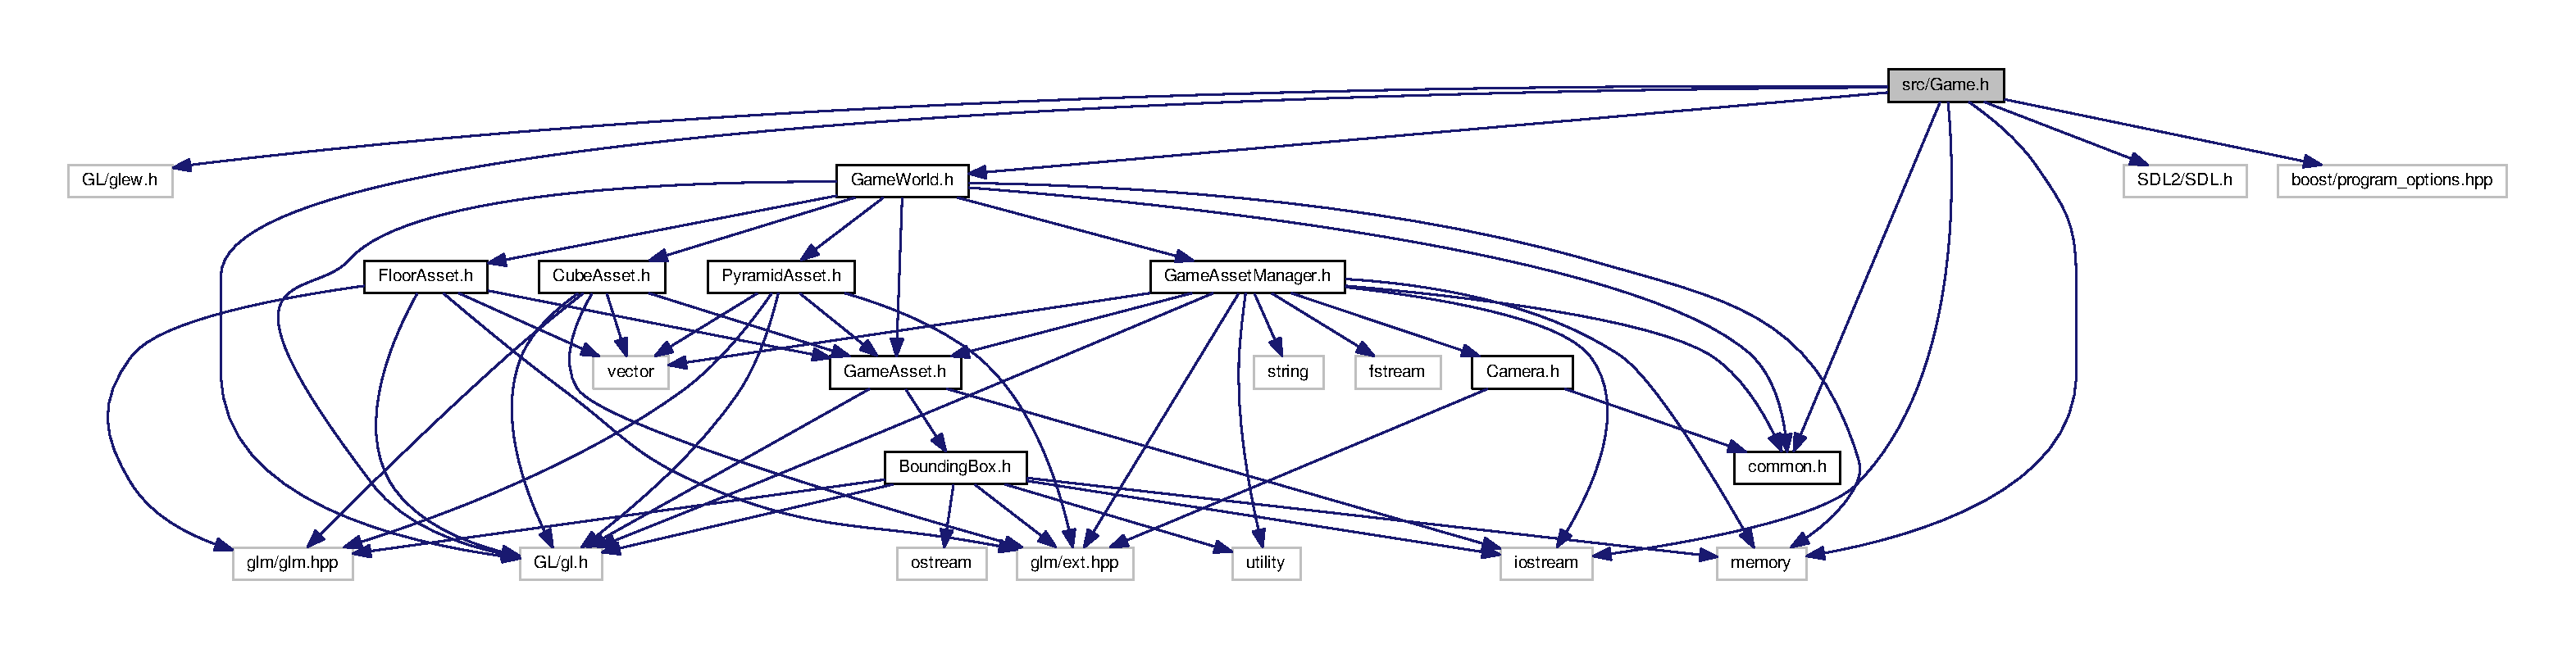
\includegraphics[width=350pt]{_game_8h__incl}
\end{center}
\end{figure}
This graph shows which files directly or indirectly include this file\+:\nopagebreak
\begin{figure}[H]
\begin{center}
\leavevmode
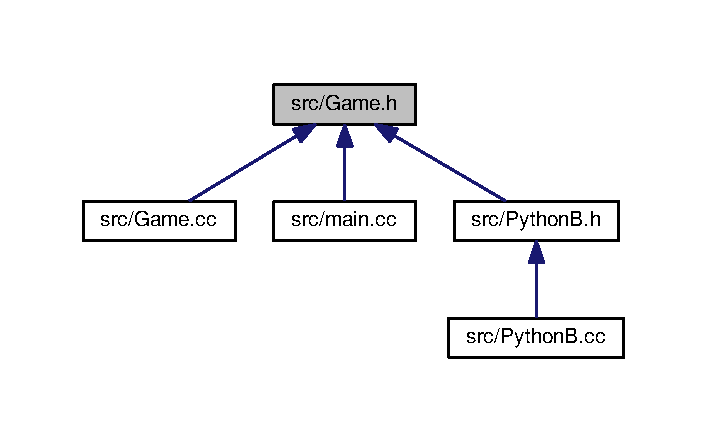
\includegraphics[width=340pt]{_game_8h__dep__incl}
\end{center}
\end{figure}
\subsection*{Classes}
\begin{DoxyCompactItemize}
\item 
class \hyperlink{class_game}{Game}
\end{DoxyCompactItemize}

\hypertarget{_game_asset_8cc}{}\section{src/\+Game\+Asset.cc File Reference}
\label{_game_asset_8cc}\index{src/\+Game\+Asset.\+cc@{src/\+Game\+Asset.\+cc}}
{\ttfamily \#include \char`\"{}Game\+Asset.\+h\char`\"{}}\\*
Include dependency graph for Game\+Asset.\+cc\+:
\nopagebreak
\begin{figure}[H]
\begin{center}
\leavevmode
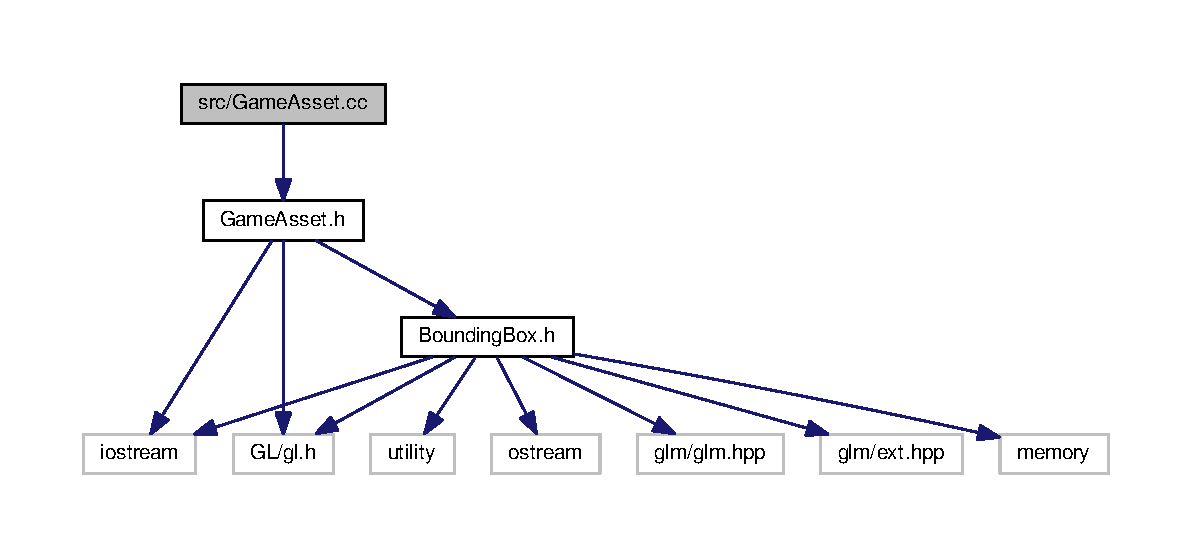
\includegraphics[width=350pt]{_game_asset_8cc__incl}
\end{center}
\end{figure}

\hypertarget{_game_asset_8h}{}\section{src/\+Game\+Asset.h File Reference}
\label{_game_asset_8h}\index{src/\+Game\+Asset.\+h@{src/\+Game\+Asset.\+h}}
{\ttfamily \#include $<$iostream$>$}\\*
{\ttfamily \#include $<$G\+L/gl.\+h$>$}\\*
{\ttfamily \#include \char`\"{}Bounding\+Box.\+h\char`\"{}}\\*
Include dependency graph for Game\+Asset.\+h\+:
\nopagebreak
\begin{figure}[H]
\begin{center}
\leavevmode
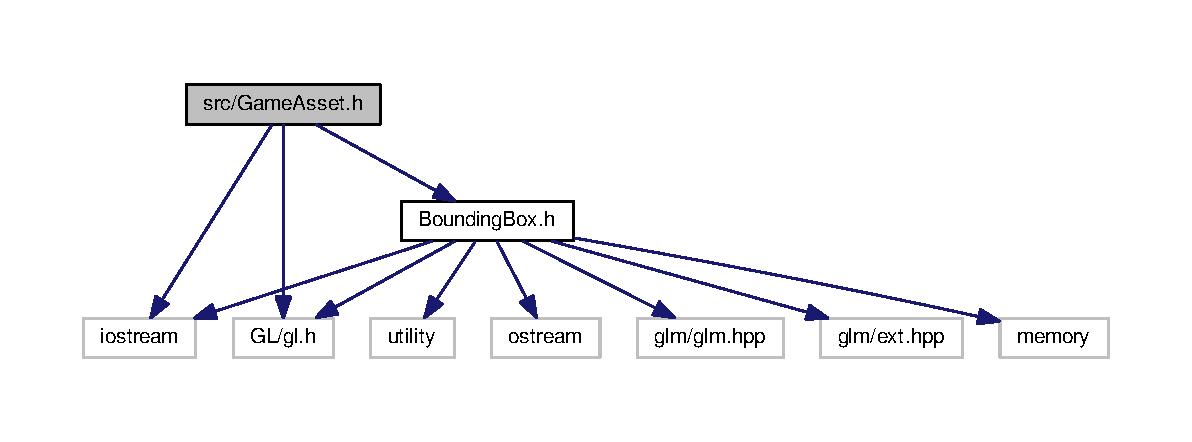
\includegraphics[width=350pt]{_game_asset_8h__incl}
\end{center}
\end{figure}
This graph shows which files directly or indirectly include this file\+:
\nopagebreak
\begin{figure}[H]
\begin{center}
\leavevmode
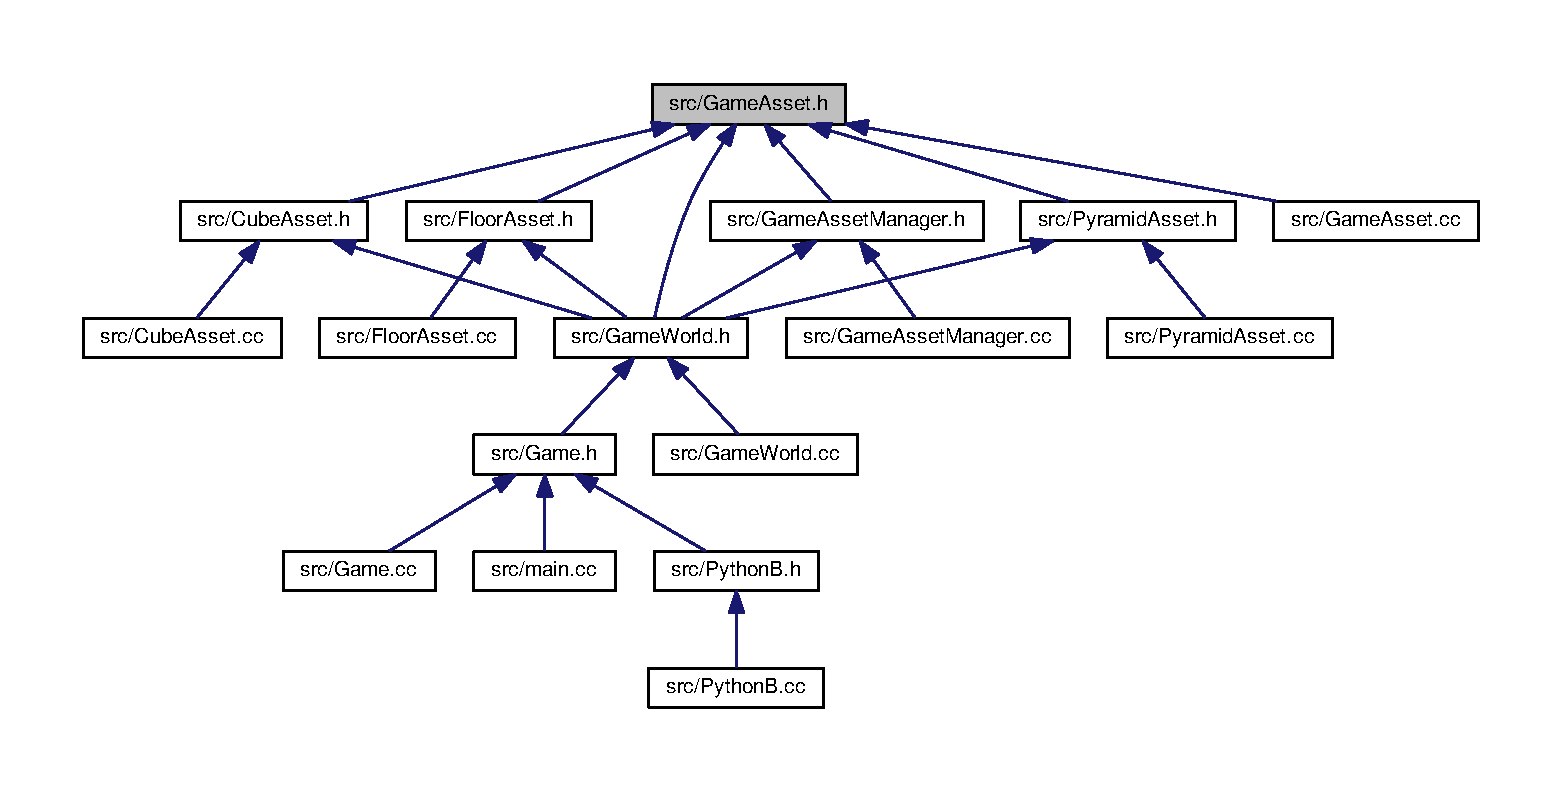
\includegraphics[width=350pt]{_game_asset_8h__dep__incl}
\end{center}
\end{figure}
\subsection*{Classes}
\begin{DoxyCompactItemize}
\item 
class \hyperlink{class_game_asset}{Game\+Asset}
\end{DoxyCompactItemize}

\hypertarget{_game_asset_manager_8cc}{}\section{src/\+Game\+Asset\+Manager.cc File Reference}
\label{_game_asset_manager_8cc}\index{src/\+Game\+Asset\+Manager.\+cc@{src/\+Game\+Asset\+Manager.\+cc}}
{\ttfamily \#include \char`\"{}Game\+Asset\+Manager.\+h\char`\"{}}\\*
Include dependency graph for Game\+Asset\+Manager.\+cc\+:\nopagebreak
\begin{figure}[H]
\begin{center}
\leavevmode
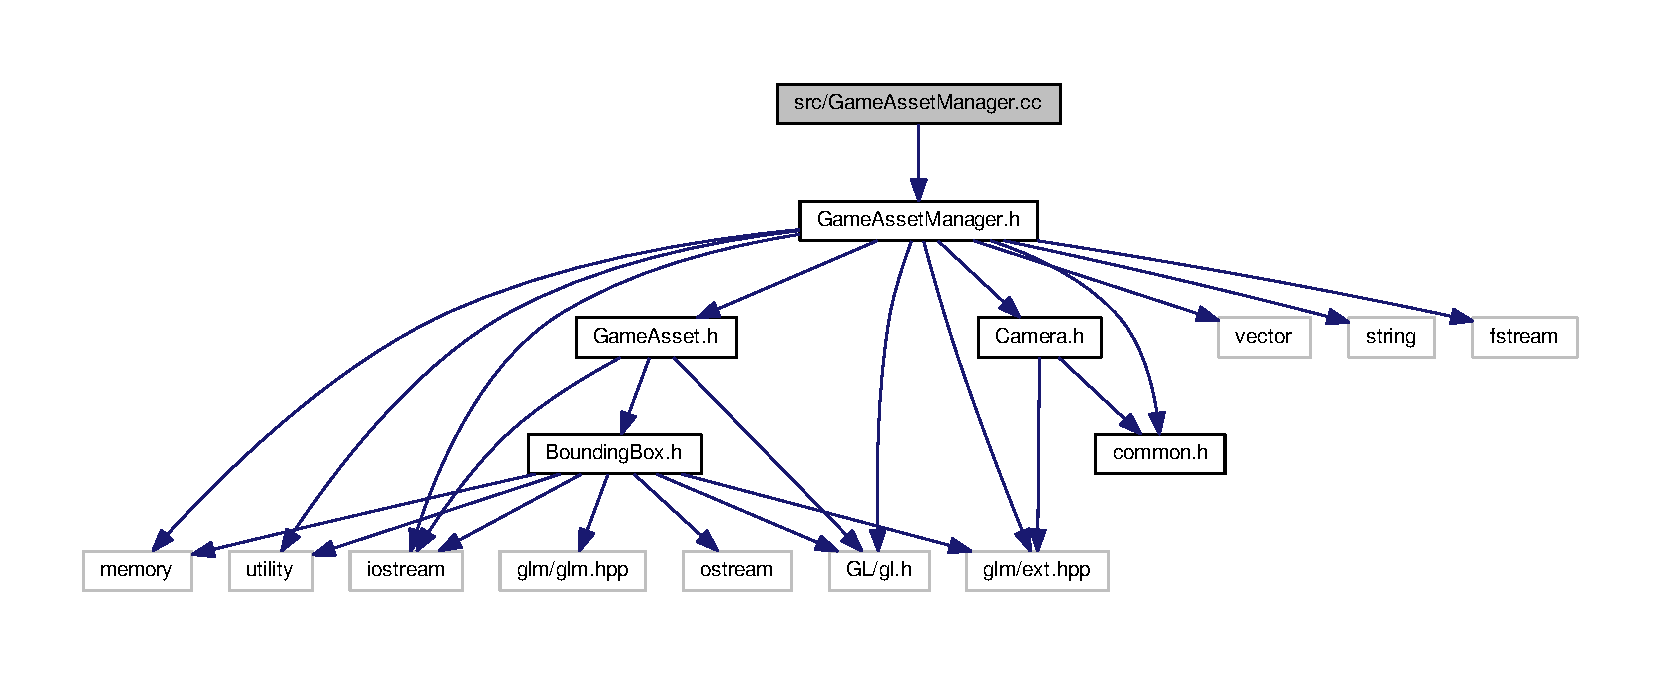
\includegraphics[width=350pt]{_game_asset_manager_8cc__incl}
\end{center}
\end{figure}

\hypertarget{_game_asset_manager_8h}{}\section{src/\+Game\+Asset\+Manager.h File Reference}
\label{_game_asset_manager_8h}\index{src/\+Game\+Asset\+Manager.\+h@{src/\+Game\+Asset\+Manager.\+h}}
{\ttfamily \#include $<$memory$>$}\\*
{\ttfamily \#include $<$vector$>$}\\*
{\ttfamily \#include $<$string$>$}\\*
{\ttfamily \#include $<$utility$>$}\\*
{\ttfamily \#include $<$fstream$>$}\\*
{\ttfamily \#include $<$iostream$>$}\\*
{\ttfamily \#include $<$G\+L/gl.\+h$>$}\\*
{\ttfamily \#include $<$glm/ext.\+hpp$>$}\\*
{\ttfamily \#include \char`\"{}common.\+h\char`\"{}}\\*
{\ttfamily \#include \char`\"{}Game\+Asset.\+h\char`\"{}}\\*
{\ttfamily \#include \char`\"{}Camera.\+h\char`\"{}}\\*
Include dependency graph for Game\+Asset\+Manager.\+h\+:
\nopagebreak
\begin{figure}[H]
\begin{center}
\leavevmode
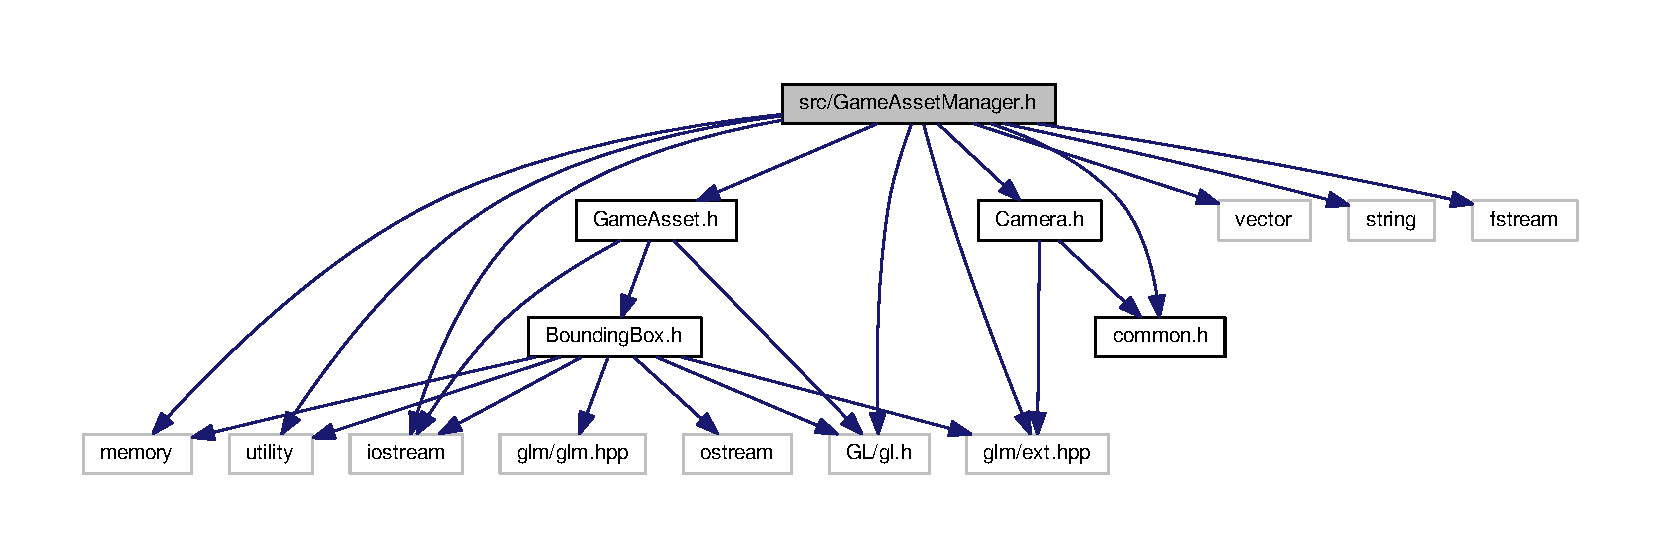
\includegraphics[width=350pt]{_game_asset_manager_8h__incl}
\end{center}
\end{figure}
This graph shows which files directly or indirectly include this file\+:
\nopagebreak
\begin{figure}[H]
\begin{center}
\leavevmode
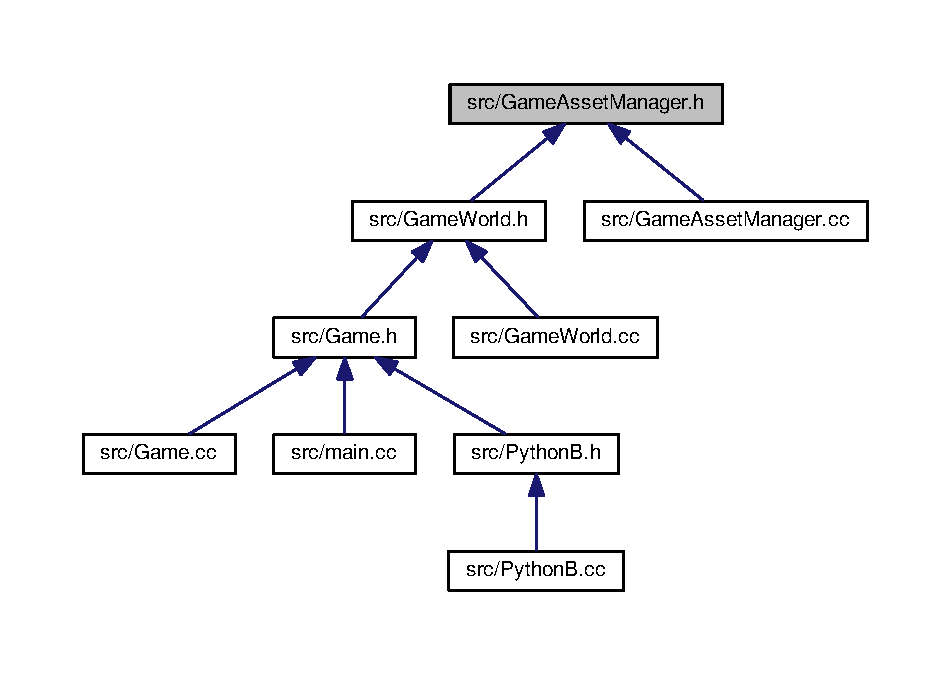
\includegraphics[width=350pt]{_game_asset_manager_8h__dep__incl}
\end{center}
\end{figure}
\subsection*{Classes}
\begin{DoxyCompactItemize}
\item 
class \hyperlink{class_game_asset_manager}{Game\+Asset\+Manager}
\end{DoxyCompactItemize}

\hypertarget{_game_world_8cc}{}\section{src/\+Game\+World.cc File Reference}
\label{_game_world_8cc}\index{src/\+Game\+World.\+cc@{src/\+Game\+World.\+cc}}
{\ttfamily \#include \char`\"{}Game\+World.\+h\char`\"{}}\\*
Include dependency graph for Game\+World.\+cc\+:\nopagebreak
\begin{figure}[H]
\begin{center}
\leavevmode
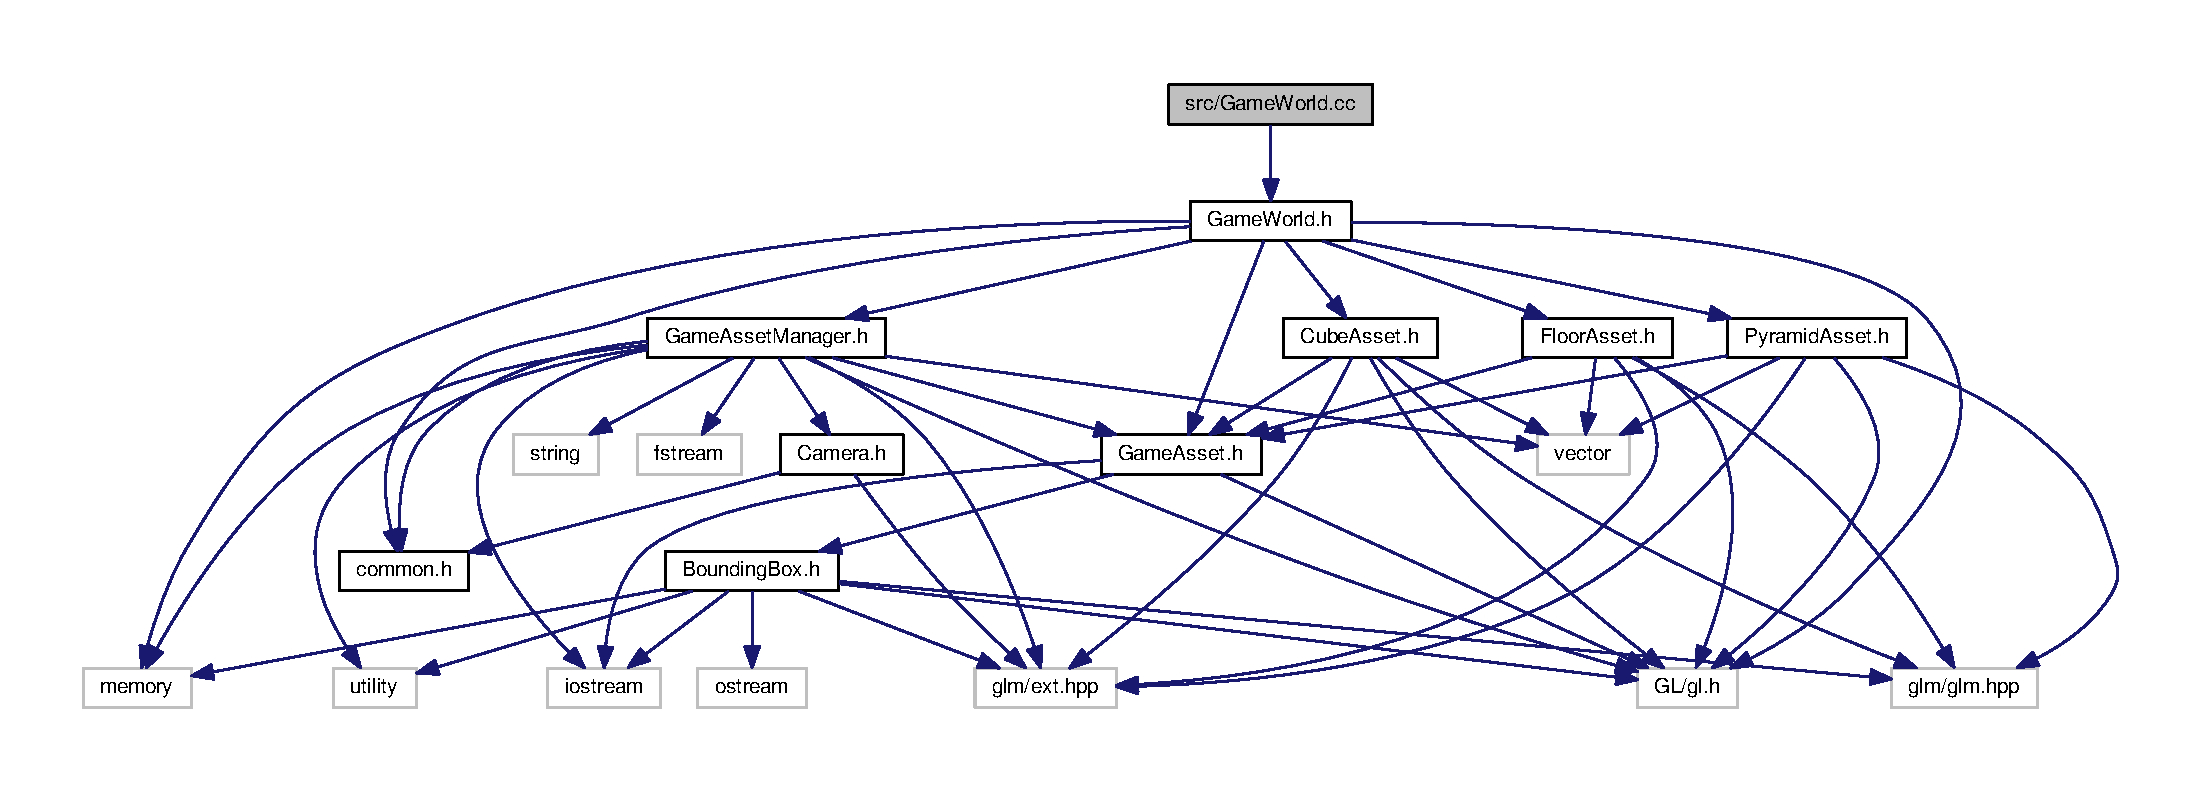
\includegraphics[width=350pt]{_game_world_8cc__incl}
\end{center}
\end{figure}

\hypertarget{_game_world_8h}{}\section{src/\+Game\+World.h File Reference}
\label{_game_world_8h}\index{src/\+Game\+World.\+h@{src/\+Game\+World.\+h}}
{\ttfamily \#include $<$memory$>$}\\*
{\ttfamily \#include $<$G\+L/gl.\+h$>$}\\*
{\ttfamily \#include \char`\"{}common.\+h\char`\"{}}\\*
{\ttfamily \#include \char`\"{}Game\+Asset\+Manager.\+h\char`\"{}}\\*
{\ttfamily \#include \char`\"{}Game\+Asset.\+h\char`\"{}}\\*
{\ttfamily \#include \char`\"{}Cube\+Asset.\+h\char`\"{}}\\*
{\ttfamily \#include \char`\"{}Floor\+Asset.\+h\char`\"{}}\\*
{\ttfamily \#include \char`\"{}Pyramid\+Asset.\+h\char`\"{}}\\*
Include dependency graph for Game\+World.\+h\+:
\nopagebreak
\begin{figure}[H]
\begin{center}
\leavevmode
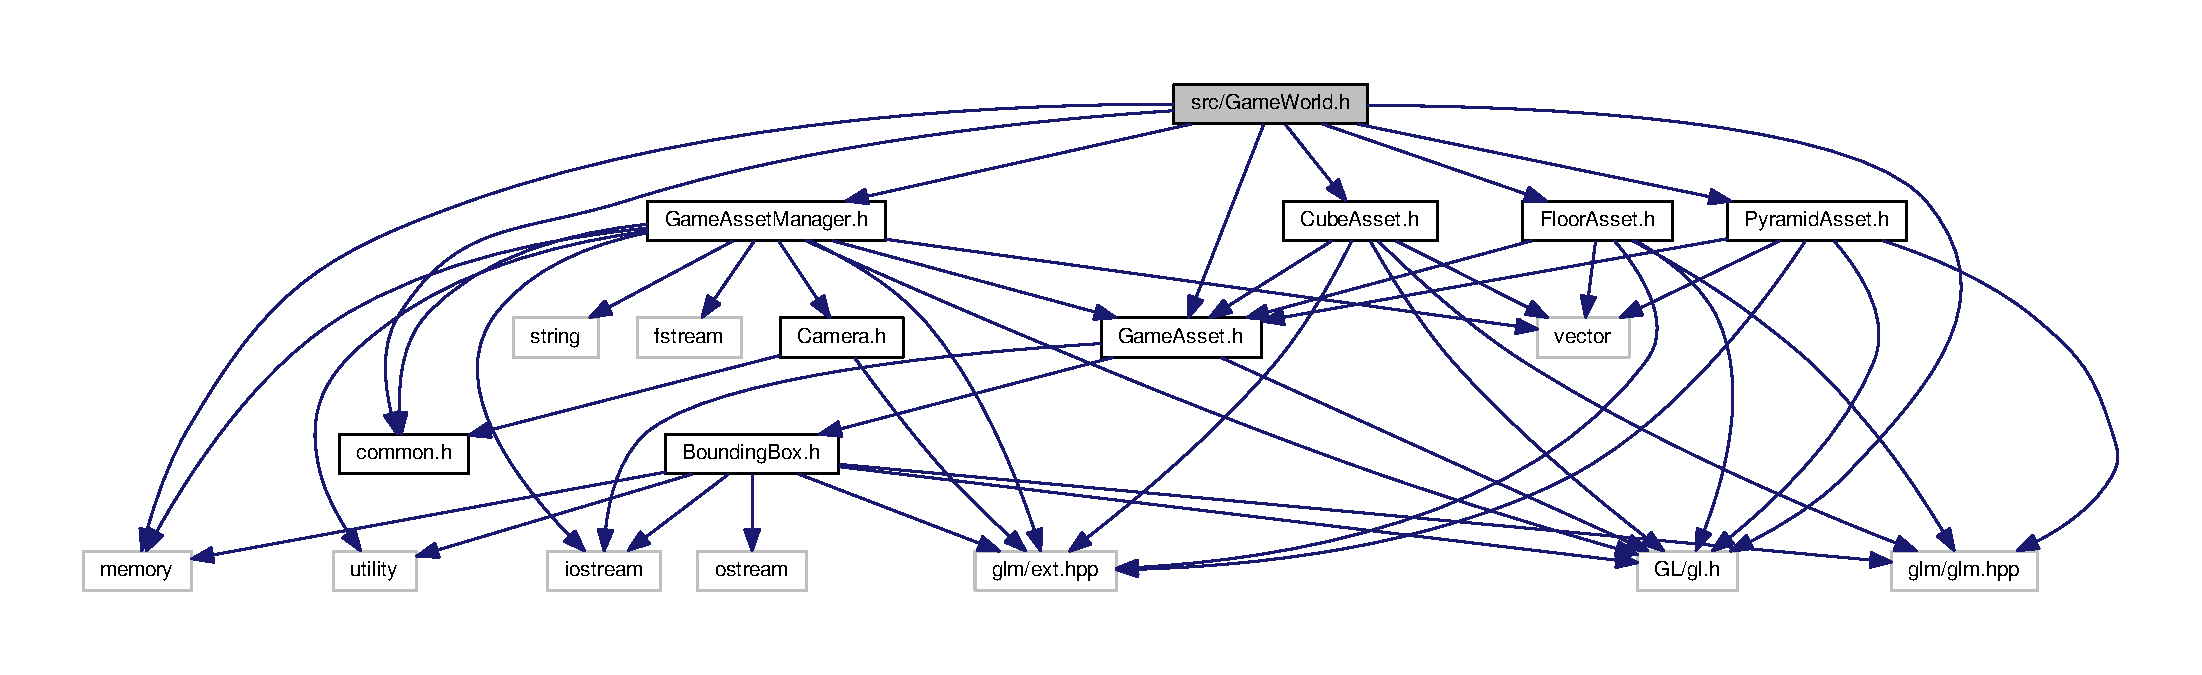
\includegraphics[width=350pt]{_game_world_8h__incl}
\end{center}
\end{figure}
This graph shows which files directly or indirectly include this file\+:
\nopagebreak
\begin{figure}[H]
\begin{center}
\leavevmode
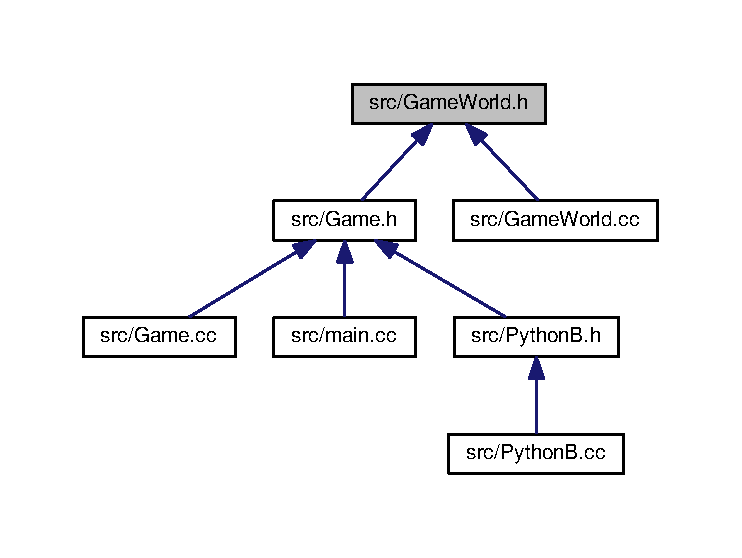
\includegraphics[width=350pt]{_game_world_8h__dep__incl}
\end{center}
\end{figure}
\subsection*{Classes}
\begin{DoxyCompactItemize}
\item 
class \hyperlink{class_game_world}{Game\+World}
\end{DoxyCompactItemize}

\hypertarget{main_8cc}{}\section{src/main.cc File Reference}
\label{main_8cc}\index{src/main.\+cc@{src/main.\+cc}}
{\ttfamily \#include \char`\"{}Game.\+h\char`\"{}}\\*
Include dependency graph for main.\+cc\+:
\nopagebreak
\begin{figure}[H]
\begin{center}
\leavevmode
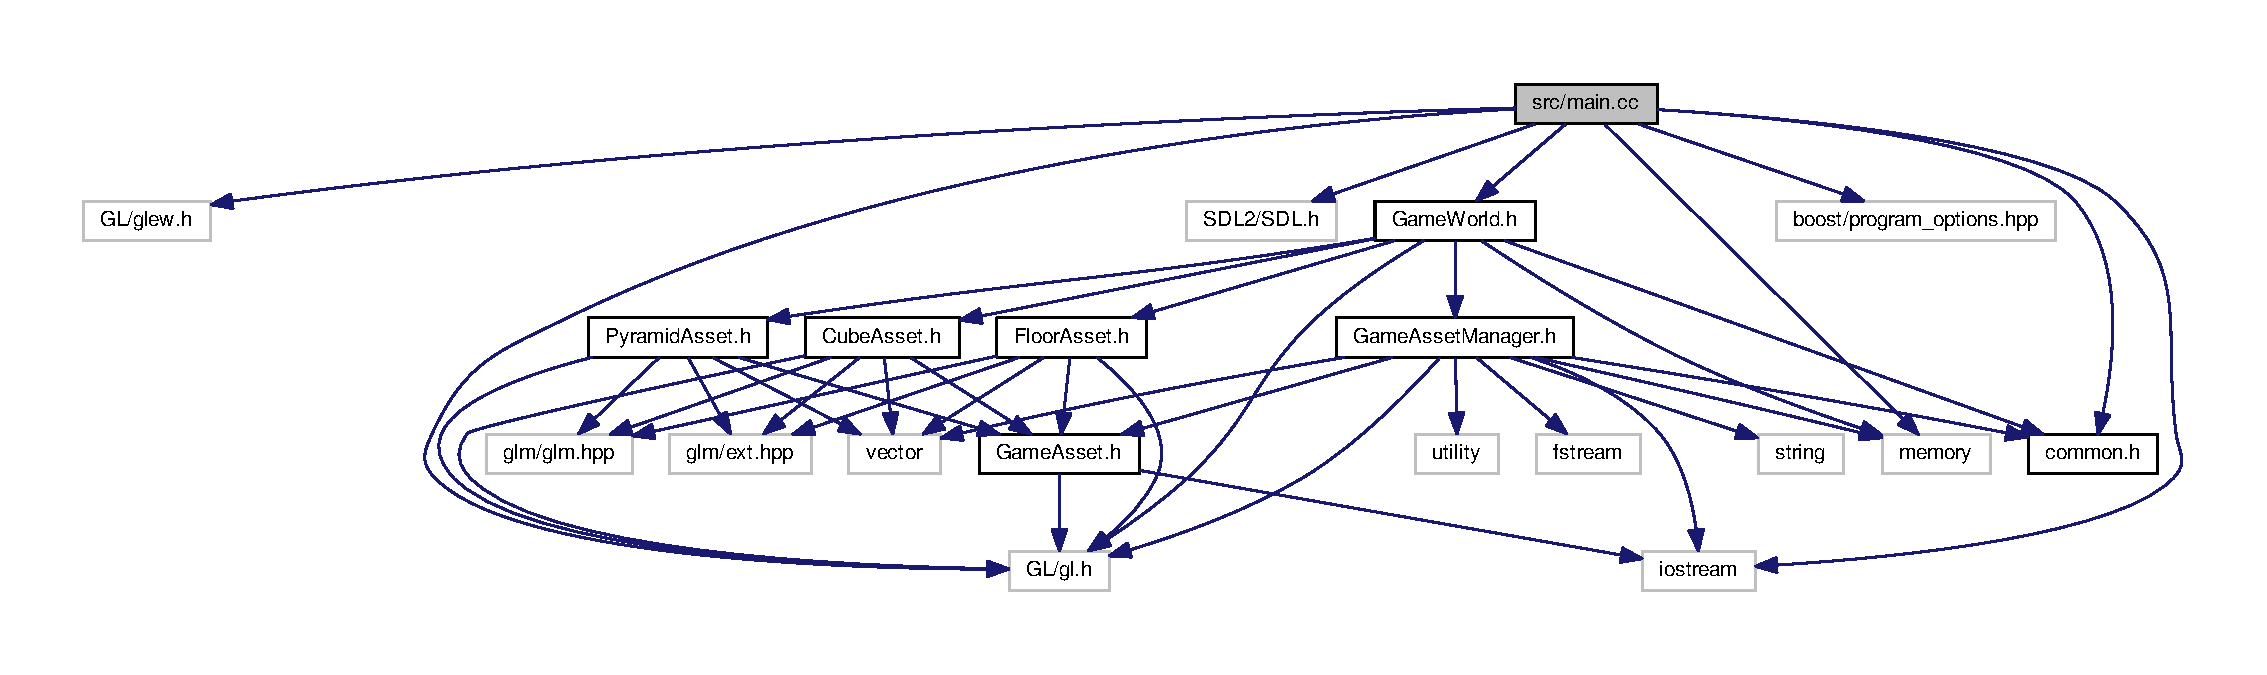
\includegraphics[width=350pt]{main_8cc__incl}
\end{center}
\end{figure}
\subsection*{Functions}
\begin{DoxyCompactItemize}
\item 
int \hyperlink{main_8cc_ae66f6b31b5ad750f1fe042a706a4e3d4}{main} ()
\end{DoxyCompactItemize}


\subsection{Function Documentation}
\hypertarget{main_8cc_ae66f6b31b5ad750f1fe042a706a4e3d4}{}\index{main.\+cc@{main.\+cc}!main@{main}}
\index{main@{main}!main.\+cc@{main.\+cc}}
\subsubsection[{main()}]{\setlength{\rightskip}{0pt plus 5cm}int main (
\begin{DoxyParamCaption}
{}
\end{DoxyParamCaption}
)}\label{main_8cc_ae66f6b31b5ad750f1fe042a706a4e3d4}
Main Runs the \hyperlink{class_game}{Game} file which handles the main loop of the game. 
\hypertarget{_pyramid_asset_8cc}{}\section{src/\+Pyramid\+Asset.cc File Reference}
\label{_pyramid_asset_8cc}\index{src/\+Pyramid\+Asset.\+cc@{src/\+Pyramid\+Asset.\+cc}}
{\ttfamily \#include \char`\"{}Pyramid\+Asset.\+h\char`\"{}}\\*
Include dependency graph for Pyramid\+Asset.\+cc\+:
\nopagebreak
\begin{figure}[H]
\begin{center}
\leavevmode
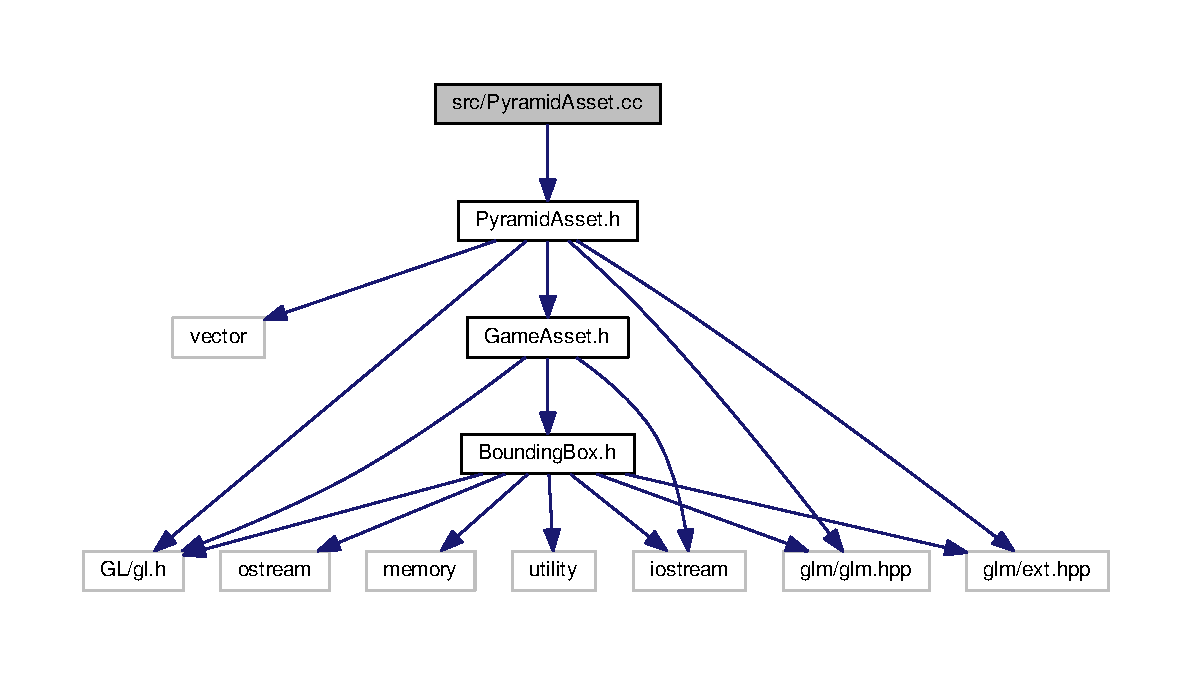
\includegraphics[width=350pt]{_pyramid_asset_8cc__incl}
\end{center}
\end{figure}
\subsection*{Macros}
\begin{DoxyCompactItemize}
\item 
\#define \hyperlink{_pyramid_asset_8cc_a75f201b0e53e68726854997957322b8d}{check\+G\+L\+Error}()
\end{DoxyCompactItemize}


\subsection{Macro Definition Documentation}
\hypertarget{_pyramid_asset_8cc_a75f201b0e53e68726854997957322b8d}{}\index{Pyramid\+Asset.\+cc@{Pyramid\+Asset.\+cc}!check\+G\+L\+Error@{check\+G\+L\+Error}}
\index{check\+G\+L\+Error@{check\+G\+L\+Error}!Pyramid\+Asset.\+cc@{Pyramid\+Asset.\+cc}}
\subsubsection[{check\+G\+L\+Error}]{\setlength{\rightskip}{0pt plus 5cm}\#define check\+G\+L\+Error(
\begin{DoxyParamCaption}
{}
\end{DoxyParamCaption}
)}\label{_pyramid_asset_8cc_a75f201b0e53e68726854997957322b8d}

\hypertarget{_pyramid_asset_8h}{}\section{src/\+Pyramid\+Asset.h File Reference}
\label{_pyramid_asset_8h}\index{src/\+Pyramid\+Asset.\+h@{src/\+Pyramid\+Asset.\+h}}
{\ttfamily \#include $<$vector$>$}\\*
{\ttfamily \#include $<$G\+L/gl.\+h$>$}\\*
{\ttfamily \#include $<$glm/glm.\+hpp$>$}\\*
{\ttfamily \#include $<$glm/ext.\+hpp$>$}\\*
{\ttfamily \#include \char`\"{}Game\+Asset.\+h\char`\"{}}\\*
Include dependency graph for Pyramid\+Asset.\+h\+:\nopagebreak
\begin{figure}[H]
\begin{center}
\leavevmode
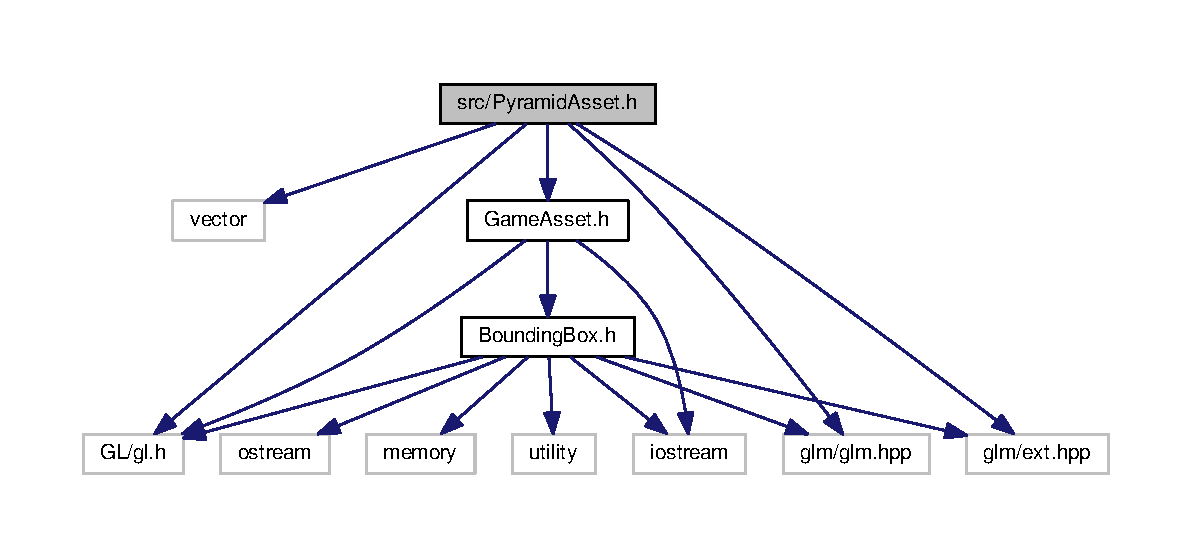
\includegraphics[width=350pt]{_pyramid_asset_8h__incl}
\end{center}
\end{figure}
This graph shows which files directly or indirectly include this file\+:\nopagebreak
\begin{figure}[H]
\begin{center}
\leavevmode
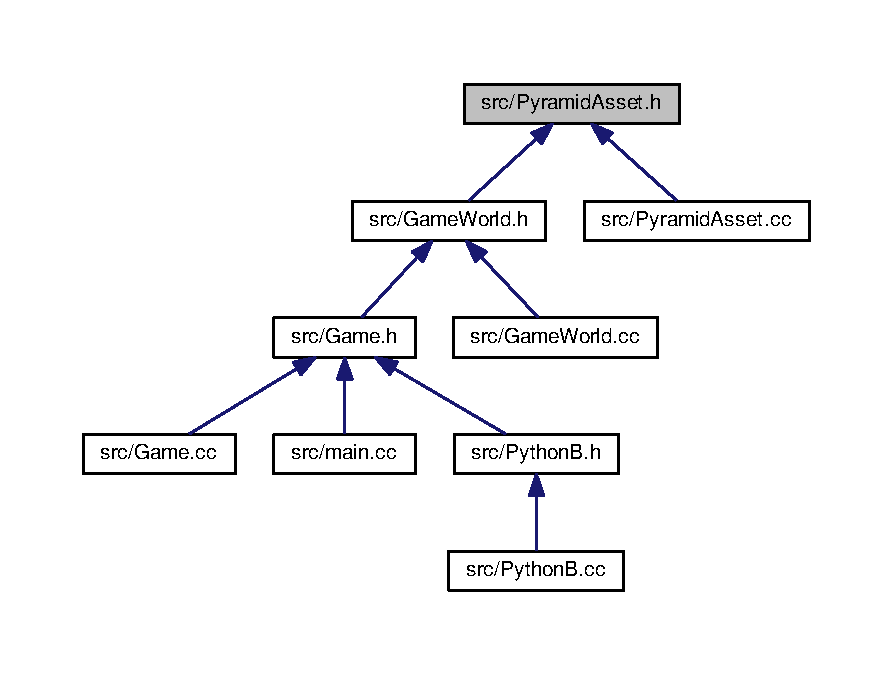
\includegraphics[width=350pt]{_pyramid_asset_8h__dep__incl}
\end{center}
\end{figure}
\subsection*{Classes}
\begin{DoxyCompactItemize}
\item 
class \hyperlink{class_pyramid_asset}{Pyramid\+Asset}
\end{DoxyCompactItemize}

\hypertarget{_python_b_8cc}{}\section{src/\+Python\+B.cc File Reference}
\label{_python_b_8cc}\index{src/\+Python\+B.\+cc@{src/\+Python\+B.\+cc}}
{\ttfamily \#include \char`\"{}Python\+B.\+h\char`\"{}}\\*
Include dependency graph for Python\+B.\+cc\+:\nopagebreak
\begin{figure}[H]
\begin{center}
\leavevmode
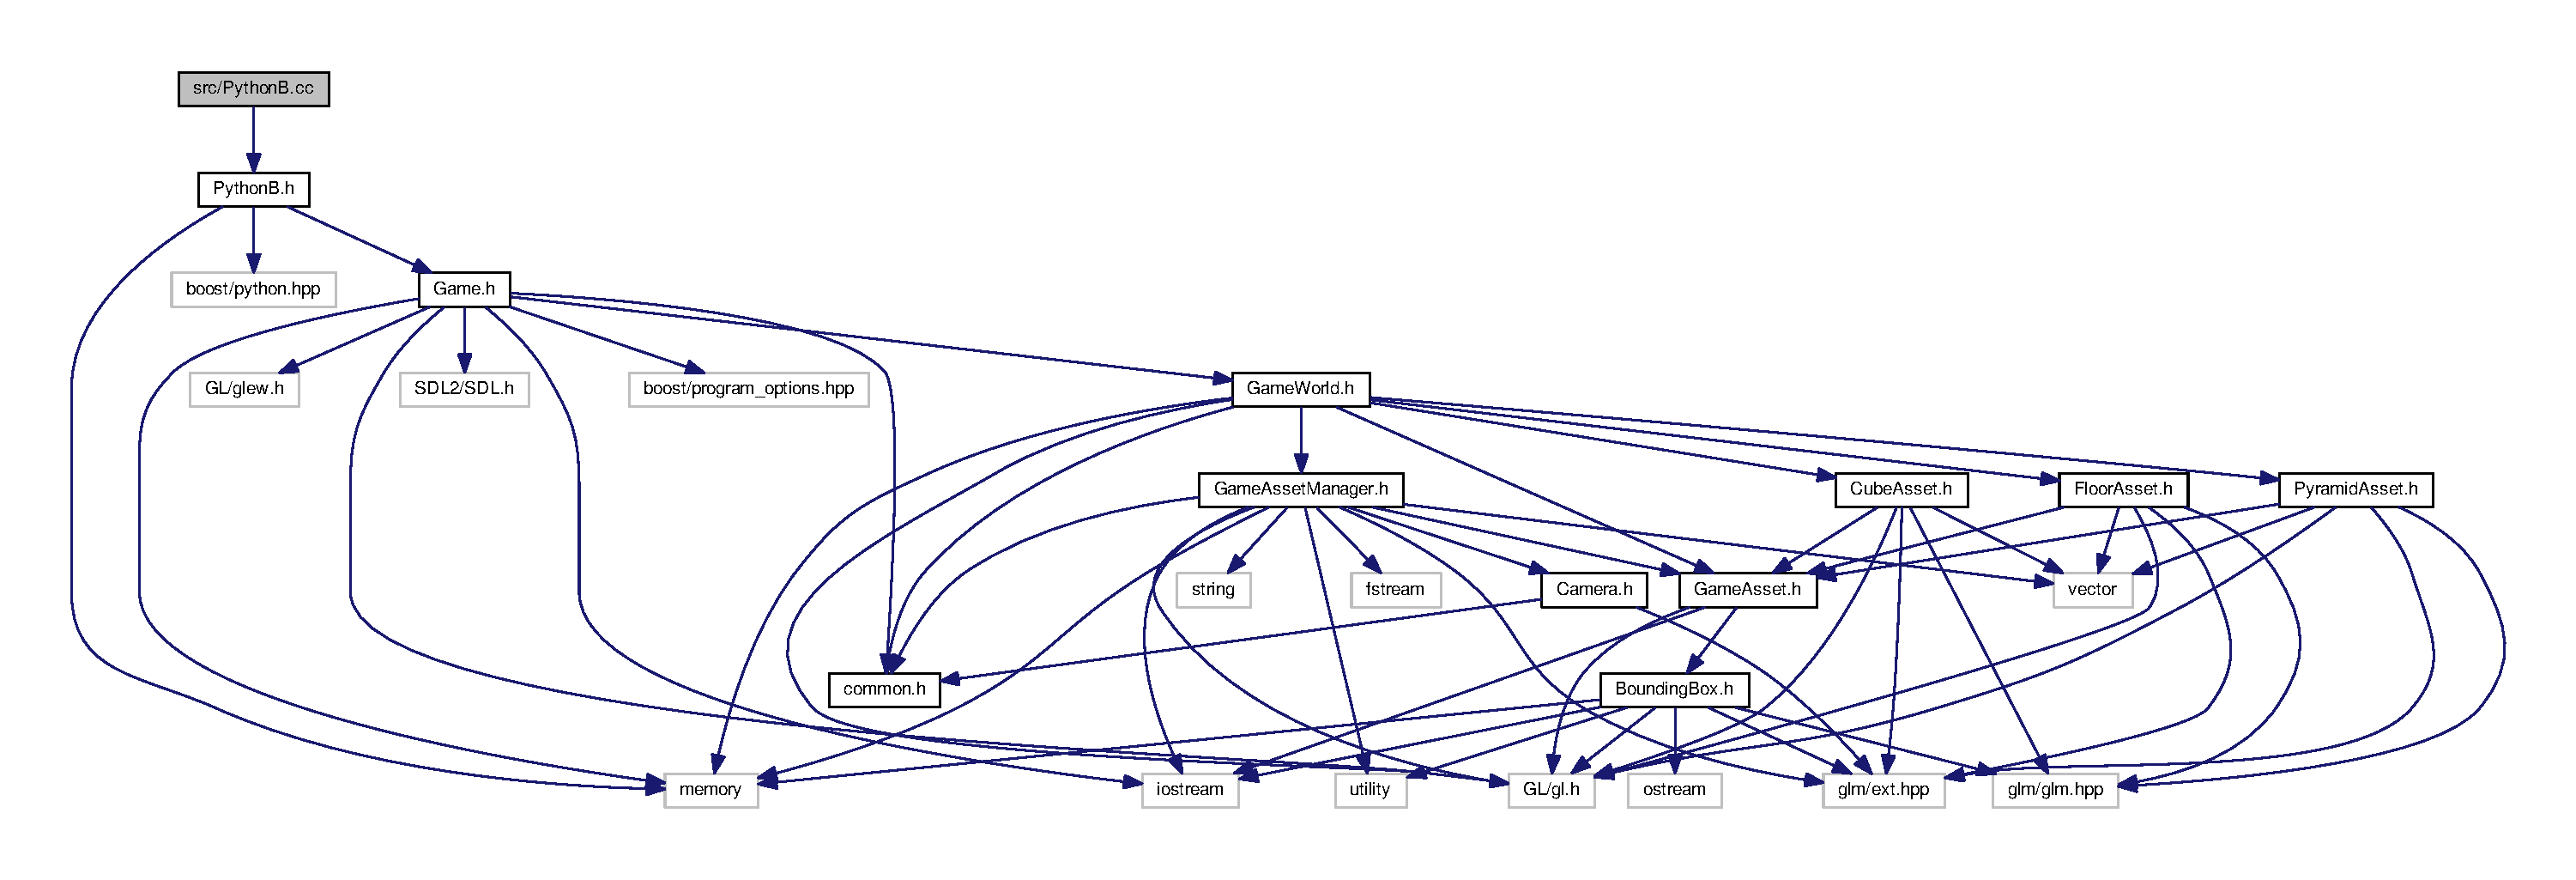
\includegraphics[width=350pt]{_python_b_8cc__incl}
\end{center}
\end{figure}
\subsection*{Functions}
\begin{DoxyCompactItemize}
\item 
char const $\ast$ \hyperlink{_python_b_8cc_a53ccbad24d8da8192f3d47407feb6cd8}{hello} ()
\item 
\hyperlink{_python_b_8cc_a031ba5ba3eea9a8da1bcd110d089a888}{B\+O\+O\+S\+T\+\_\+\+P\+Y\+T\+H\+O\+N\+\_\+\+M\+O\+D\+U\+L\+E} (liblink)
\end{DoxyCompactItemize}


\subsection{Function Documentation}
\hypertarget{_python_b_8cc_a031ba5ba3eea9a8da1bcd110d089a888}{}\index{Python\+B.\+cc@{Python\+B.\+cc}!B\+O\+O\+S\+T\+\_\+\+P\+Y\+T\+H\+O\+N\+\_\+\+M\+O\+D\+U\+L\+E@{B\+O\+O\+S\+T\+\_\+\+P\+Y\+T\+H\+O\+N\+\_\+\+M\+O\+D\+U\+L\+E}}
\index{B\+O\+O\+S\+T\+\_\+\+P\+Y\+T\+H\+O\+N\+\_\+\+M\+O\+D\+U\+L\+E@{B\+O\+O\+S\+T\+\_\+\+P\+Y\+T\+H\+O\+N\+\_\+\+M\+O\+D\+U\+L\+E}!Python\+B.\+cc@{Python\+B.\+cc}}
\subsubsection[{B\+O\+O\+S\+T\+\_\+\+P\+Y\+T\+H\+O\+N\+\_\+\+M\+O\+D\+U\+L\+E(liblink)}]{\setlength{\rightskip}{0pt plus 5cm}B\+O\+O\+S\+T\+\_\+\+P\+Y\+T\+H\+O\+N\+\_\+\+M\+O\+D\+U\+L\+E (
\begin{DoxyParamCaption}
\item[{liblink}]{}
\end{DoxyParamCaption}
)}\label{_python_b_8cc_a031ba5ba3eea9a8da1bcd110d089a888}


Here is the call graph for this function\+:\nopagebreak
\begin{figure}[H]
\begin{center}
\leavevmode
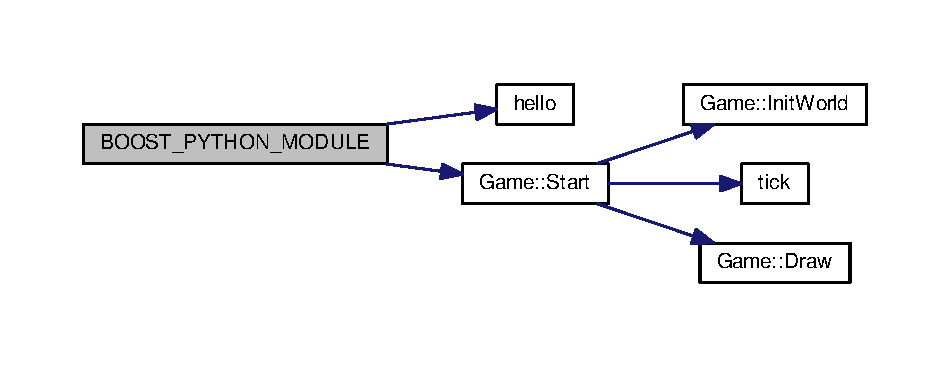
\includegraphics[width=350pt]{_python_b_8cc_a031ba5ba3eea9a8da1bcd110d089a888_cgraph}
\end{center}
\end{figure}


\hypertarget{_python_b_8cc_a53ccbad24d8da8192f3d47407feb6cd8}{}\index{Python\+B.\+cc@{Python\+B.\+cc}!hello@{hello}}
\index{hello@{hello}!Python\+B.\+cc@{Python\+B.\+cc}}
\subsubsection[{hello()}]{\setlength{\rightskip}{0pt plus 5cm}char const$\ast$ hello (
\begin{DoxyParamCaption}
{}
\end{DoxyParamCaption}
)}\label{_python_b_8cc_a53ccbad24d8da8192f3d47407feb6cd8}


Here is the caller graph for this function\+:\nopagebreak
\begin{figure}[H]
\begin{center}
\leavevmode
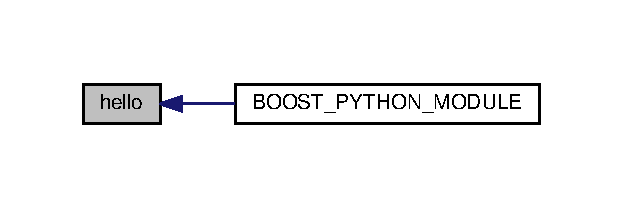
\includegraphics[width=299pt]{_python_b_8cc_a53ccbad24d8da8192f3d47407feb6cd8_icgraph}
\end{center}
\end{figure}



\hypertarget{_python_b_8h}{}\section{src/\+Python\+B.h File Reference}
\label{_python_b_8h}\index{src/\+Python\+B.\+h@{src/\+Python\+B.\+h}}
{\ttfamily \#include $<$memory$>$}\\*
{\ttfamily \#include $<$boost/python.\+hpp$>$}\\*
{\ttfamily \#include \char`\"{}Game.\+h\char`\"{}}\\*
Include dependency graph for Python\+B.\+h\+:
\nopagebreak
\begin{figure}[H]
\begin{center}
\leavevmode
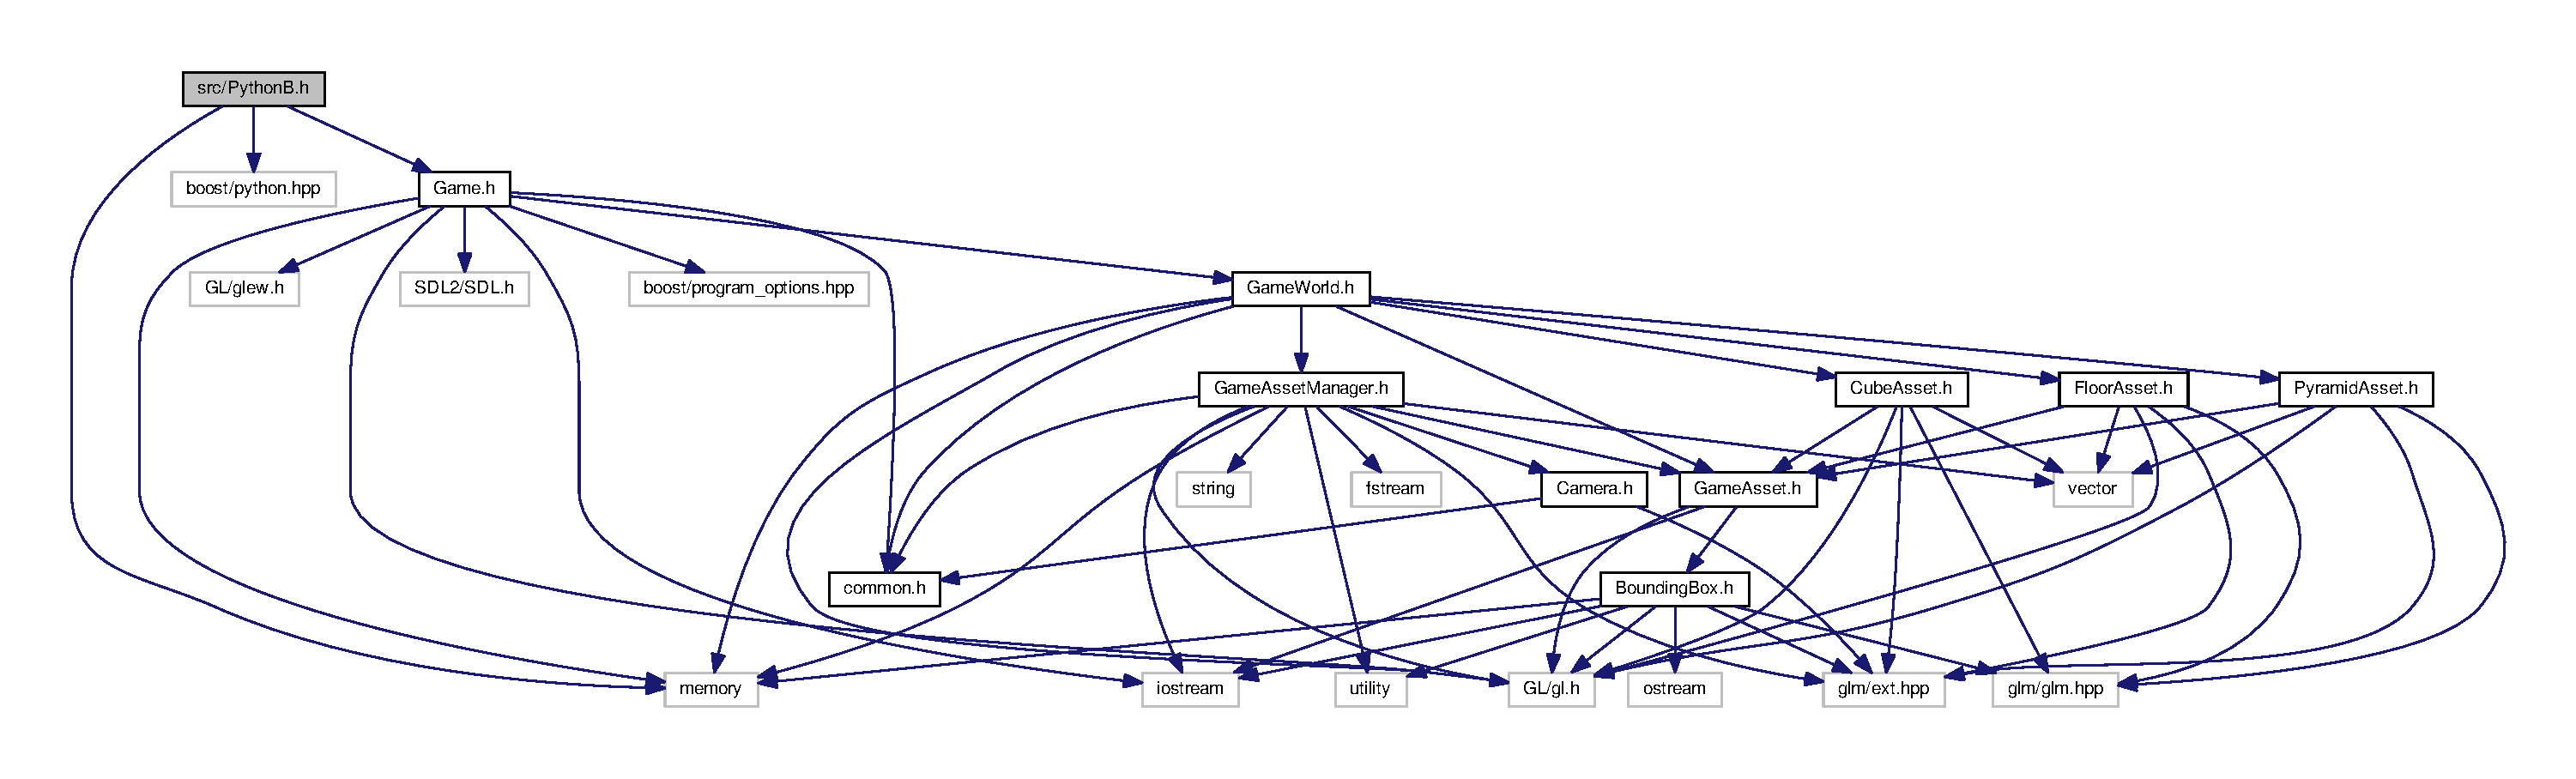
\includegraphics[width=350pt]{_python_b_8h__incl}
\end{center}
\end{figure}
This graph shows which files directly or indirectly include this file\+:
\nopagebreak
\begin{figure}[H]
\begin{center}
\leavevmode
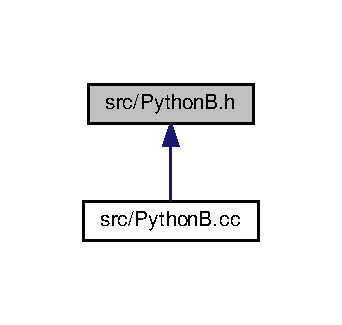
\includegraphics[width=164pt]{_python_b_8h__dep__incl}
\end{center}
\end{figure}
\subsection*{Classes}
\begin{DoxyCompactItemize}
\item 
class \hyperlink{class_python_b}{Python\+B}
\end{DoxyCompactItemize}

\hypertarget{_python_b_8py}{}\section{src/\+Python\+B.py File Reference}
\label{_python_b_8py}\index{src/\+Python\+B.\+py@{src/\+Python\+B.\+py}}
\subsection*{Namespaces}
\begin{DoxyCompactItemize}
\item 
 \hyperlink{namespace_python_b}{Python\+B}
\end{DoxyCompactItemize}

%--- End generated contents ---

% Index
\backmatter
\newpage
\phantomsection
\clearemptydoublepage
\addcontentsline{toc}{chapter}{Index}
\printindex

\end{document}
